\documentclass[USenglish,cleveref, autoref, thm-restate]{lipics-v2019}
\usepackage{listings,hyperref,multirow,paralist,xspace,url}
\newcommand{\missingTag}[1]{\textcolor{red}{#1}\xspace}
\newcommand{\missingNumber}{\textcolor{red}{XX}\xspace}
\newcommand{\missingPercentage}{\textcolor{red}{XX\%}\xspace}
\newcommand{\missingTable}[1][XX]{\textcolor{red}{Table #1}\xspace}
\newcommand{\missingGraph}{\textcolor{red}{XXGraph}\xspace}


%\newcommand{\CoreEvalCallCountRnd}{12.6M\xspace}
\newcommand{\CoreEvalCallCount}{12,637,139\xspace}
\newcommand{\CoreEvalSiteCountRnd}{170\xspace}
\newcommand{\CoreEvalSiteCount}{170\xspace}
\newcommand{\CoreEvalParentCallCountRnd}{254.1K\xspace}
\newcommand{\CoreEvalParentCallCount}{254,112\xspace}
\newcommand{\CoreEvalParentSiteCountRnd}{16\xspace}
\newcommand{\CoreEvalParentSiteCount}{16\xspace}
\newcommand{\CoreEvalqCallCountRnd}{265.5K\xspace}
\newcommand{\CoreEvalqCallCount}{265,499\xspace}
\newcommand{\CoreEvalqSiteCountRnd}{4\xspace}
\newcommand{\CoreEvalqSiteCount}{4\xspace}
\newcommand{\CoreLocalCallCountRnd}{234.2K\xspace}
\newcommand{\CoreLocalCallCount}{234,212\xspace}
\newcommand{\CoreLocalSiteCountRnd}{1.1K\xspace}
\newcommand{\CoreLocalSiteCount}{1,116\xspace}
\newcommand{\PackageEvalCallCountRnd}{5M\xspace}
\newcommand{\PackageEvalCallCount}{5,021,240\xspace}
\newcommand{\PackageEvalSiteCountRnd}{2.4K\xspace}
\newcommand{\PackageEvalSiteCount}{2,448\xspace}
\newcommand{\PackageEvalParentCallCountRnd}{52.1K\xspace}
\newcommand{\PackageEvalParentCallCount}{52,130\xspace}
\newcommand{\PackageEvalParentSiteCountRnd}{351\xspace}
\newcommand{\PackageEvalParentSiteCount}{351\xspace}
\newcommand{\PackageEvalqCallCountRnd}{292\xspace}
\newcommand{\PackageEvalqCallCount}{292\xspace}
\newcommand{\PackageEvalqSiteCountRnd}{7\xspace}
\newcommand{\PackageEvalqSiteCount}{7\xspace}
\newcommand{\PackageLocalCallCountRnd}{1.3K\xspace}
\newcommand{\PackageLocalCallCount}{1,251\xspace}
\newcommand{\PackageLocalSiteCountRnd}{8\xspace}
\newcommand{\PackageLocalSiteCount}{8\xspace}
\newcommand{\KaggleEvalCallCountRnd}{0\xspace}
\newcommand{\KaggleEvalCallCount}{0\xspace}
\newcommand{\KaggleEvalSiteCountRnd}{0\xspace}
\newcommand{\KaggleEvalSiteCount}{0\xspace}
\newcommand{\KaggleEvalParentCallCountRnd}{0\xspace}
\newcommand{\KaggleEvalParentCallCount}{0\xspace}
\newcommand{\KaggleEvalParentSiteCountRnd}{0\xspace}
\newcommand{\KaggleEvalParentSiteCount}{0\xspace}
\newcommand{\KaggleEvalqCallCountRnd}{0\xspace}
\newcommand{\KaggleEvalqCallCount}{0\xspace}
\newcommand{\KaggleEvalqSiteCountRnd}{0\xspace}
\newcommand{\KaggleEvalqSiteCount}{0\xspace}
\newcommand{\KaggleLocalCallCountRnd}{0\xspace}
\newcommand{\KaggleLocalCallCount}{0\xspace}
\newcommand{\KaggleLocalSiteCountRnd}{0\xspace}
\newcommand{\KaggleLocalSiteCount}{0\xspace}
\newcommand{\CoreAllCallCountRnd}{13.4M\xspace}
\newcommand{\CoreAllCallCount}{13,390,962\xspace}
\newcommand{\CoreAllSiteCountRnd}{1.3K\xspace}
\newcommand{\CoreAllSiteCount}{1,306\xspace}
\newcommand{\KaggleAllCallCountRnd}{0\xspace}
\newcommand{\KaggleAllCallCount}{0\xspace}
\newcommand{\KaggleAllSiteCountRnd}{0\xspace}
\newcommand{\KaggleAllSiteCount}{0\xspace}
\newcommand{\PackageAllCallCountRnd}{5.1M\xspace}
\newcommand{\PackageAllCallCount}{5,074,913\xspace}
\newcommand{\PackageAllSiteCountRnd}{2.8K\xspace}
\newcommand{\PackageAllSiteCount}{2,814\xspace}
\newcommand{\AllEvalCallCountRnd}{17.7M\xspace}
\newcommand{\AllEvalCallCount}{17,658,379\xspace}
\newcommand{\AllEvalSiteCountRnd}{2.6K\xspace}
\newcommand{\AllEvalSiteCount}{2,618\xspace}
\newcommand{\AllEvalParentCallCountRnd}{306.2K\xspace}
\newcommand{\AllEvalParentCallCount}{306,242\xspace}
\newcommand{\AllEvalParentSiteCountRnd}{367\xspace}
\newcommand{\AllEvalParentSiteCount}{367\xspace}
\newcommand{\AllEvalqCallCountRnd}{265.8K\xspace}
\newcommand{\AllEvalqCallCount}{265,791\xspace}
\newcommand{\AllEvalqSiteCountRnd}{11\xspace}
\newcommand{\AllEvalqSiteCount}{11\xspace}
\newcommand{\AllLocalCallCountRnd}{235.5K\xspace}
\newcommand{\AllLocalCallCount}{235,463\xspace}
\newcommand{\AllLocalSiteCountRnd}{1.1K\xspace}
\newcommand{\AllLocalSiteCount}{1,124\xspace}
\newcommand{\AllAllCallCountRnd}{18.5M\xspace}
\newcommand{\AllAllCallCount}{18,465,875\xspace}
\newcommand{\AllAllSiteCountRnd}{4.1K\xspace}
\newcommand{\AllAllSiteCount}{4,120\xspace}
\newcommand{\TotalFileCountRnd}{23.9K\xspace}
\newcommand{\TotalFileCount}{23,871\xspace}
\newcommand{\NoEvalFileCountRnd}{0\xspace}
\newcommand{\NoEvalFileCount}{0\xspace}
\newcommand{\NoEvalFilePerc}{0\%\xspace}
\newcommand{\CoreEvalFileCountRnd}{13.6K\xspace}
\newcommand{\CoreEvalFileCount}{13,584\xspace}
\newcommand{\CoreEvalFilePerc}{56.9\%\xspace}
\newcommand{\PackageEvalFileCountRnd}{224\xspace}
\newcommand{\PackageEvalFileCount}{224\xspace}
\newcommand{\PackageEvalFilePerc}{0.9\%\xspace}
\newcommand{\AllEvalFileCountRnd}{10.1K\xspace}
\newcommand{\AllEvalFileCount}{10,063\xspace}
\newcommand{\AllEvalFilePerc}{42.2\%\xspace}
\newcommand{\EightyCoreEvalFileCountRnd}{5.9K\xspace}
\newcommand{\EightyCoreEvalFileCount}{5,930\xspace}
\newcommand{\EightyCoreEvalFilePerc}{58.9\%\xspace}
\newcommand{\TopTenPackageCallCountRnd}{3.8M\xspace}
\newcommand{\TopTenPackageCallCount}{3,794,346\xspace}
\newcommand{\TopTenPackageCallPerc}{86.5\%\xspace}
\newcommand{\TopTenPackageSiteCountRnd}{169\xspace}
\newcommand{\TopTenPackageSiteCount}{169\xspace}
\newcommand{\TopTenPackageSitePerc}{6.2\%\xspace}
\newcommand{\TopTenPackageNameA}{ggplot2\xspace}
\newcommand{\TopTenPackageCallsiteCountARnd}{2\xspace}
\newcommand{\TopTenPackageCallsiteCountA}{2\xspace}
\newcommand{\TopTenPackageCallCountARnd}{2M\xspace}
\newcommand{\TopTenPackageCallCountA}{2,026,739\xspace}
\newcommand{\TopTenPackageCallPercA}{46.2\%\xspace}
\newcommand{\TopTenPackageNameB}{magrittr\xspace}
\newcommand{\TopTenPackageCallsiteCountBRnd}{6\xspace}
\newcommand{\TopTenPackageCallsiteCountB}{6\xspace}
\newcommand{\TopTenPackageCallCountBRnd}{536K\xspace}
\newcommand{\TopTenPackageCallCountB}{536,016\xspace}
\newcommand{\TopTenPackageCallPercB}{12.2\%\xspace}
\newcommand{\TopTenPackageNameC}{data.table\xspace}
\newcommand{\TopTenPackageCallsiteCountCRnd}{47\xspace}
\newcommand{\TopTenPackageCallsiteCountC}{47\xspace}
\newcommand{\TopTenPackageCallCountCRnd}{229.1K\xspace}
\newcommand{\TopTenPackageCallCountC}{229,073\xspace}
\newcommand{\TopTenPackageCallPercC}{5.2\%\xspace}
\newcommand{\TopTenPackageNameD}{glue\xspace}
\newcommand{\TopTenPackageCallsiteCountDRnd}{9\xspace}
\newcommand{\TopTenPackageCallsiteCountD}{9\xspace}
\newcommand{\TopTenPackageCallCountDRnd}{192.4K\xspace}
\newcommand{\TopTenPackageCallCountD}{192,423\xspace}
\newcommand{\TopTenPackageCallPercD}{4.4\%\xspace}
\newcommand{\TopTenPackageNameE}{brms\xspace}
\newcommand{\TopTenPackageCallsiteCountERnd}{1\xspace}
\newcommand{\TopTenPackageCallsiteCountE}{1\xspace}
\newcommand{\TopTenPackageCallCountERnd}{166.1K\xspace}
\newcommand{\TopTenPackageCallCountE}{166,132\xspace}
\newcommand{\TopTenPackageCallPercE}{3.8\%\xspace}
\newcommand{\TopTenPackageNameF}{copula\xspace}
\newcommand{\TopTenPackageCallsiteCountFRnd}{52\xspace}
\newcommand{\TopTenPackageCallsiteCountF}{52\xspace}
\newcommand{\TopTenPackageCallCountFRnd}{145.8K\xspace}
\newcommand{\TopTenPackageCallCountF}{145,762\xspace}
\newcommand{\TopTenPackageCallPercF}{3.3\%\xspace}
\newcommand{\TopTenPackageNameG}{np\xspace}
\newcommand{\TopTenPackageCallsiteCountGRnd}{23\xspace}
\newcommand{\TopTenPackageCallsiteCountG}{23\xspace}
\newcommand{\TopTenPackageCallCountGRnd}{142K\xspace}
\newcommand{\TopTenPackageCallCountG}{141,967\xspace}
\newcommand{\TopTenPackageCallPercG}{3.2\%\xspace}
\newcommand{\TopTenPackageNameH}{R6\xspace}
\newcommand{\TopTenPackageCallsiteCountHRnd}{1\xspace}
\newcommand{\TopTenPackageCallsiteCountH}{1\xspace}
\newcommand{\TopTenPackageCallCountHRnd}{128.4K\xspace}
\newcommand{\TopTenPackageCallCountH}{128,371\xspace}
\newcommand{\TopTenPackageCallPercH}{2.9\%\xspace}
\newcommand{\TopTenPackageNameI}{plyr\xspace}
\newcommand{\TopTenPackageCallsiteCountIRnd}{17\xspace}
\newcommand{\TopTenPackageCallsiteCountI}{17\xspace}
\newcommand{\TopTenPackageCallCountIRnd}{118.4K\xspace}
\newcommand{\TopTenPackageCallCountI}{118,408\xspace}
\newcommand{\TopTenPackageCallPercI}{2.7\%\xspace}
\newcommand{\TopTenPackageNameJ}{statnet.common\xspace}
\newcommand{\TopTenPackageCallsiteCountJRnd}{11\xspace}
\newcommand{\TopTenPackageCallsiteCountJ}{11\xspace}
\newcommand{\TopTenPackageCallCountJRnd}{109.5K\xspace}
\newcommand{\TopTenPackageCallCountJ}{109,455\xspace}
\newcommand{\TopTenPackageCallPercJ}{2.5\%\xspace}
\newcommand{\SiteSummarySiteCountA}{1\xspace}
\newcommand{\SiteSummaryPackageCountARnd}{89\xspace}
\newcommand{\SiteSummaryPackageCountA}{89\xspace}
\newcommand{\SiteSummarySiteCountB}{2\xspace}
\newcommand{\SiteSummaryPackageCountBRnd}{41\xspace}
\newcommand{\SiteSummaryPackageCountB}{41\xspace}
\newcommand{\SiteSummarySiteCountC}{3\xspace}
\newcommand{\SiteSummaryPackageCountCRnd}{23\xspace}
\newcommand{\SiteSummaryPackageCountC}{23\xspace}
\newcommand{\SiteSummarySiteCountD}{4\xspace}
\newcommand{\SiteSummaryPackageCountDRnd}{19\xspace}
\newcommand{\SiteSummaryPackageCountD}{19\xspace}
\newcommand{\SiteSummarySiteCountE}{5\xspace}
\newcommand{\SiteSummaryPackageCountERnd}{11\xspace}
\newcommand{\SiteSummaryPackageCountE}{11\xspace}
\newcommand{\SiteSummarySiteCountF}{6\xspace}
\newcommand{\SiteSummaryPackageCountFRnd}{20\xspace}
\newcommand{\SiteSummaryPackageCountF}{20\xspace}
\newcommand{\SiteSummarySiteCountG}{7\xspace}
\newcommand{\SiteSummaryPackageCountGRnd}{15\xspace}
\newcommand{\SiteSummaryPackageCountG}{15\xspace}
\newcommand{\SiteSummarySiteCountH}{8\xspace}
\newcommand{\SiteSummaryPackageCountHRnd}{3\xspace}
\newcommand{\SiteSummaryPackageCountH}{3\xspace}
\newcommand{\SiteSummarySiteCountI}{9\xspace}
\newcommand{\SiteSummaryPackageCountIRnd}{7\xspace}
\newcommand{\SiteSummaryPackageCountI}{7\xspace}
\newcommand{\SiteSummarySiteCountJ}{10\xspace}
\newcommand{\SiteSummaryPackageCountJRnd}{3\xspace}
\newcommand{\SiteSummaryPackageCountJ}{3\xspace}
\newcommand{\SiteSummarySiteCountK}{> 200\xspace}
\newcommand{\SiteSummaryPackageCountKRnd}{1\xspace}
\newcommand{\SiteSummaryPackageCountK}{1\xspace}
\newcommand{\SiteSummarySiteCountL}{101150\xspace}
\newcommand{\SiteSummaryPackageCountLRnd}{2\xspace}
\newcommand{\SiteSummaryPackageCountL}{2\xspace}
\newcommand{\SiteSummarySiteCountM}{1150\xspace}
\newcommand{\SiteSummaryPackageCountMRnd}{39\xspace}
\newcommand{\SiteSummaryPackageCountM}{39\xspace}
\newcommand{\SiteSummarySiteCountN}{151200\xspace}
\newcommand{\SiteSummaryPackageCountNRnd}{1\xspace}
\newcommand{\SiteSummaryPackageCountN}{1\xspace}
\newcommand{\SiteSummarySiteCountO}{51100\xspace}
\newcommand{\SiteSummaryPackageCountORnd}{7\xspace}
\newcommand{\SiteSummaryPackageCountO}{7\xspace}
\newcommand{\DegreeMonomorphism}{89.2\%\xspace}

\newcommand{\CoreEvalCallCountRnd}{6.3M\xspace}
\newcommand{\CoreEvalCallCount}{6,282,429\xspace}
\newcommand{\CoreEvalSiteCountRnd}{185\xspace}
\newcommand{\CoreEvalSiteCount}{185\xspace}
\newcommand{\CoreEvalParentCallCountRnd}{186K\xspace}
\newcommand{\CoreEvalParentCallCount}{186,275\xspace}
\newcommand{\CoreEvalParentSiteCountRnd}{13\xspace}
\newcommand{\CoreEvalParentSiteCount}{13\xspace}
\newcommand{\CoreEvalqCallCountRnd}{132K\xspace}
\newcommand{\CoreEvalqCallCount}{132,891\xspace}
\newcommand{\CoreEvalqSiteCountRnd}{20K\xspace}
\newcommand{\CoreEvalqSiteCount}{20,460\xspace}
\newcommand{\CoreLocalCallCountRnd}{175K\xspace}
\newcommand{\CoreLocalCallCount}{175,079\xspace}
\newcommand{\CoreLocalSiteCountRnd}{920\xspace}
\newcommand{\CoreLocalSiteCount}{920\xspace}
\newcommand{\PackageEvalCallCountRnd}{1.6M\xspace}
\newcommand{\PackageEvalCallCount}{1,582,738\xspace}
\newcommand{\PackageEvalSiteCountRnd}{1.5K\xspace}
\newcommand{\PackageEvalSiteCount}{1,459\xspace}
\newcommand{\PackageEvalParentCallCountRnd}{13K\xspace}
\newcommand{\PackageEvalParentCallCount}{13,230\xspace}
\newcommand{\PackageEvalParentSiteCountRnd}{249\xspace}
\newcommand{\PackageEvalParentSiteCount}{249\xspace}
\newcommand{\PackageEvalqCallCountRnd}{2\xspace}
\newcommand{\PackageEvalqCallCount}{2\xspace}
\newcommand{\PackageEvalqSiteCountRnd}{1\xspace}
\newcommand{\PackageEvalqSiteCount}{1\xspace}
\newcommand{\PackageLocalCallCountRnd}{2.2K\xspace}
\newcommand{\PackageLocalCallCount}{2,228\xspace}
\newcommand{\PackageLocalSiteCountRnd}{15\xspace}
\newcommand{\PackageLocalSiteCount}{15\xspace}
\newcommand{\KaggleEvalCallCountRnd}{0\xspace}
\newcommand{\KaggleEvalCallCount}{0\xspace}
\newcommand{\KaggleEvalSiteCountRnd}{0\xspace}
\newcommand{\KaggleEvalSiteCount}{0\xspace}
\newcommand{\KaggleEvalParentCallCountRnd}{0\xspace}
\newcommand{\KaggleEvalParentCallCount}{0\xspace}
\newcommand{\KaggleEvalParentSiteCountRnd}{0\xspace}
\newcommand{\KaggleEvalParentSiteCount}{0\xspace}
\newcommand{\KaggleEvalqCallCountRnd}{0\xspace}
\newcommand{\KaggleEvalqCallCount}{0\xspace}
\newcommand{\KaggleEvalqSiteCountRnd}{0\xspace}
\newcommand{\KaggleEvalqSiteCount}{0\xspace}
\newcommand{\KaggleLocalCallCountRnd}{0\xspace}
\newcommand{\KaggleLocalCallCount}{0\xspace}
\newcommand{\KaggleLocalSiteCountRnd}{0\xspace}
\newcommand{\KaggleLocalSiteCount}{0\xspace}
\newcommand{\CoreAllCallCountRnd}{6.8M\xspace}
\newcommand{\CoreAllCallCount}{6,776,674\xspace}
\newcommand{\CoreAllSiteCountRnd}{21.6K\xspace}
\newcommand{\CoreAllSiteCount}{21,578\xspace}
\newcommand{\KaggleAllCallCountRnd}{0\xspace}
\newcommand{\KaggleAllCallCount}{0\xspace}
\newcommand{\KaggleAllSiteCountRnd}{0\xspace}
\newcommand{\KaggleAllSiteCount}{0\xspace}
\newcommand{\PackageAllCallCountRnd}{1.6M\xspace}
\newcommand{\PackageAllCallCount}{1,598,198\xspace}
\newcommand{\PackageAllSiteCountRnd}{1.7K\xspace}
\newcommand{\PackageAllSiteCount}{1,724\xspace}
\newcommand{\AllEvalCallCountRnd}{7.9M\xspace}
\newcommand{\AllEvalCallCount}{7,865,167\xspace}
\newcommand{\AllEvalSiteCountRnd}{1.6K\xspace}
\newcommand{\AllEvalSiteCount}{1,644\xspace}
\newcommand{\AllEvalParentCallCountRnd}{199.5K\xspace}
\newcommand{\AllEvalParentCallCount}{199,505\xspace}
\newcommand{\AllEvalParentSiteCountRnd}{262\xspace}
\newcommand{\AllEvalParentSiteCount}{262\xspace}
\newcommand{\AllEvalqCallCountRnd}{132.9K\xspace}
\newcommand{\AllEvalqCallCount}{132,893\xspace}
\newcommand{\AllEvalqSiteCountRnd}{20.5K\xspace}
\newcommand{\AllEvalqSiteCount}{20,461\xspace}
\newcommand{\AllLocalCallCountRnd}{177.3K\xspace}
\newcommand{\AllLocalCallCount}{177,307\xspace}
\newcommand{\AllLocalSiteCountRnd}{935\xspace}
\newcommand{\AllLocalSiteCount}{935\xspace}
\newcommand{\AllAllCallCountRnd}{8.4M\xspace}
\newcommand{\AllAllCallCount}{8,374,872\xspace}
\newcommand{\AllAllSiteCountRnd}{23.3K\xspace}
\newcommand{\AllAllSiteCount}{23,302\xspace}
\newcommand{\TotalFileCountRnd}{18.3K\xspace}
\newcommand{\TotalFileCount}{18,258\xspace}
\newcommand{\NoEvalFileCountRnd}{89\xspace}
\newcommand{\NoEvalFileCount}{89\xspace}
\newcommand{\NoEvalFilePerc}{0.5\%\xspace}
\newcommand{\CoreEvalFileCountRnd}{12.3K\xspace}
\newcommand{\CoreEvalFileCount}{12,307\xspace}
\newcommand{\CoreEvalFilePerc}{67.4\%\xspace}
\newcommand{\PackageEvalFileCountRnd}{0\xspace}
\newcommand{\PackageEvalFileCount}{0\xspace}
\newcommand{\PackageEvalFilePerc}{0\%\xspace}
\newcommand{\AllEvalFileCountRnd}{5.9K\xspace}
\newcommand{\AllEvalFileCount}{5,862\xspace}
\newcommand{\AllEvalFilePerc}{32.1\%\xspace}
\newcommand{\EightyCoreEvalFileCountRnd}{3.8K\xspace}
\newcommand{\EightyCoreEvalFileCount}{3,769\xspace}
\newcommand{\EightyCoreEvalFilePerc}{64.3\%\xspace}
\newcommand{\TopTenPackageCallCountRnd}{1.4M\xspace}
\newcommand{\TopTenPackageCallCount}{1,425,902\xspace}
\newcommand{\TopTenPackageCallPerc}{89.2\%\xspace}
\newcommand{\TopTenPackageSiteCountRnd}{282\xspace}
\newcommand{\TopTenPackageSiteCount}{282\xspace}
\newcommand{\TopTenPackageSitePerc}{16\%\xspace}
\newcommand{\TopTenPackageNameA}{ggplot2\xspace}
\newcommand{\TopTenPackageCallsiteCountARnd}{2\xspace}
\newcommand{\TopTenPackageCallsiteCountA}{2\xspace}
\newcommand{\TopTenPackageCallCountARnd}{987K\xspace}
\newcommand{\TopTenPackageCallCountA}{987,946\xspace}
\newcommand{\TopTenPackageCallPercA}{61\%\xspace}
\newcommand{\TopTenPackageNameB}{magrittr\xspace}
\newcommand{\TopTenPackageCallsiteCountBRnd}{5\xspace}
\newcommand{\TopTenPackageCallsiteCountB}{5\xspace}
\newcommand{\TopTenPackageCallCountBRnd}{139K\xspace}
\newcommand{\TopTenPackageCallCountB}{139,346\xspace}
\newcommand{\TopTenPackageCallPercB}{8.7\%\xspace}
\newcommand{\TopTenPackageNameC}{plyr\xspace}
\newcommand{\TopTenPackageCallsiteCountCRnd}{11\xspace}
\newcommand{\TopTenPackageCallsiteCountC}{11\xspace}
\newcommand{\TopTenPackageCallCountCRnd}{68K\xspace}
\newcommand{\TopTenPackageCallCountC}{68,671\xspace}
\newcommand{\TopTenPackageCallPercC}{4.3\%\xspace}
\newcommand{\TopTenPackageNameD}{glue\xspace}
\newcommand{\TopTenPackageCallsiteCountDRnd}{5\xspace}
\newcommand{\TopTenPackageCallsiteCountD}{5\xspace}
\newcommand{\TopTenPackageCallCountDRnd}{62K\xspace}
\newcommand{\TopTenPackageCallCountD}{62,564\xspace}
\newcommand{\TopTenPackageCallPercD}{3.9\%\xspace}
\newcommand{\TopTenPackageNameE}{data.table\xspace}
\newcommand{\TopTenPackageCallsiteCountERnd}{31\xspace}
\newcommand{\TopTenPackageCallsiteCountE}{31\xspace}
\newcommand{\TopTenPackageCallCountERnd}{47K\xspace}
\newcommand{\TopTenPackageCallCountE}{47,464\xspace}
\newcommand{\TopTenPackageCallPercE}{3\%\xspace}
\newcommand{\TopTenPackageNameF}{statnet.common\xspace}
\newcommand{\TopTenPackageCallsiteCountFRnd}{12\xspace}
\newcommand{\TopTenPackageCallsiteCountF}{12\xspace}
\newcommand{\TopTenPackageCallCountFRnd}{30K\xspace}
\newcommand{\TopTenPackageCallCountF}{30,581\xspace}
\newcommand{\TopTenPackageCallPercF}{1.9\%\xspace}
\newcommand{\TopTenPackageNameG}{VGAM\xspace}
\newcommand{\TopTenPackageCallsiteCountGRnd}{97\xspace}
\newcommand{\TopTenPackageCallsiteCountG}{97\xspace}
\newcommand{\TopTenPackageCallCountGRnd}{23K\xspace}
\newcommand{\TopTenPackageCallCountG}{23,796\xspace}
\newcommand{\TopTenPackageCallPercG}{1.5\%\xspace}
\newcommand{\TopTenPackageNameH}{copula\xspace}
\newcommand{\TopTenPackageCallsiteCountHRnd}{21\xspace}
\newcommand{\TopTenPackageCallsiteCountH}{21\xspace}
\newcommand{\TopTenPackageCallCountHRnd}{22K\xspace}
\newcommand{\TopTenPackageCallCountH}{22,794\xspace}
\newcommand{\TopTenPackageCallPercH}{1.4\%\xspace}
\newcommand{\TopTenPackageNameI}{nlme\xspace}
\newcommand{\TopTenPackageCallsiteCountIRnd}{97\xspace}
\newcommand{\TopTenPackageCallsiteCountI}{97\xspace}
\newcommand{\TopTenPackageCallCountIRnd}{21K\xspace}
\newcommand{\TopTenPackageCallCountI}{21,483\xspace}
\newcommand{\TopTenPackageCallPercI}{1.3\%\xspace}
\newcommand{\TopTenPackageNameJ}{R6\xspace}
\newcommand{\TopTenPackageCallsiteCountJRnd}{1\xspace}
\newcommand{\TopTenPackageCallsiteCountJ}{1\xspace}
\newcommand{\TopTenPackageCallCountJRnd}{21K\xspace}
\newcommand{\TopTenPackageCallCountJ}{21,257\xspace}
\newcommand{\TopTenPackageCallPercJ}{1.3\%\xspace}

\newcommand{\CorpusPackagesRnd}{500\xspace}
\newcommand{\CorpusPackages}{500\xspace}
\newcommand{\CorpusRevdepsRnd}{39.3K\xspace}
\newcommand{\CorpusRevdeps}{39,309\xspace}
\newcommand{\CorpusRevdepsMeanRnd}{78.6\xspace}
\newcommand{\CorpusRevdepsMean}{78.6\xspace}
\newcommand{\CorpusRevdepsMedianRnd}{25.5\xspace}
\newcommand{\CorpusRevdepsMedian}{25.5\xspace}
\newcommand{\CorpusRevdepsMinRnd}{10\xspace}
\newcommand{\CorpusRevdepsMin}{10\xspace}
\newcommand{\CorpusRevdepsMaxRnd}{2K\xspace}
\newcommand{\CorpusRevdepsMax}{2,000\xspace}
\newcommand{\CorpusInCranlogsRnd}{63\xspace}
\newcommand{\CorpusInCranlogs}{63\xspace}
\newcommand{\CorpusPackageProgramsRnd}{17.5K\xspace}
\newcommand{\CorpusPackagePrograms}{17,541\xspace}
\newcommand{\CorpusPackageProgramsMeanRnd}{35.1\xspace}
\newcommand{\CorpusPackageProgramsMean}{35.1\xspace}
\newcommand{\CorpusPackageProgramsMedianRnd}{20\xspace}
\newcommand{\CorpusPackageProgramsMedian}{20\xspace}
\newcommand{\CorpusPackageProgramsMinRnd}{1\xspace}
\newcommand{\CorpusPackageProgramsMin}{1\xspace}
\newcommand{\CorpusPackageProgramsMaxRnd}{528\xspace}
\newcommand{\CorpusPackageProgramsMax}{528\xspace}
\newcommand{\CorpusPackageProgramsCodeRnd}{259.1K\xspace}
\newcommand{\CorpusPackageProgramsCode}{259,079\xspace}
\newcommand{\CorpusPackageProgramsCodeMeanRnd}{518.2\xspace}
\newcommand{\CorpusPackageProgramsCodeMean}{518.2\xspace}
\newcommand{\CorpusPackageProgramsCodeMedianRnd}{251\xspace}
\newcommand{\CorpusPackageProgramsCodeMedian}{251\xspace}
\newcommand{\CorpusPackageProgramsCodeMinRnd}{1\xspace}
\newcommand{\CorpusPackageProgramsCodeMin}{1\xspace}
\newcommand{\CorpusPackageProgramsCodeMaxRnd}{6.5K\xspace}
\newcommand{\CorpusPackageProgramsCodeMax}{6,499\xspace}
\newcommand{\CorpusPackageProgramsRuntimeRnd}{95.4K\xspace}
\newcommand{\CorpusPackageProgramsRuntime}{95,361.4\xspace}
\newcommand{\CorpusPackageProgramsRuntimeMeanRnd}{190.7\xspace}
\newcommand{\CorpusPackageProgramsRuntimeMean}{190.7\xspace}
\newcommand{\CorpusPackageProgramsRuntimeMedianRnd}{81.1\xspace}
\newcommand{\CorpusPackageProgramsRuntimeMedian}{81.1\xspace}
\newcommand{\CorpusPackageProgramsRuntimeMinRnd}{0.9\xspace}
\newcommand{\CorpusPackageProgramsRuntimeMin}{0.9\xspace}
\newcommand{\CorpusPackageProgramsRuntimeMaxRnd}{2.7K\xspace}
\newcommand{\CorpusPackageProgramsRuntimeMax}{2,715.8\xspace}
\newcommand{\CorpusExamplesProgramsRnd}{15.9K\xspace}
\newcommand{\CorpusExamplesPrograms}{15,880\xspace}
\newcommand{\CorpusExamplesProgramsMeanRnd}{31.8\xspace}
\newcommand{\CorpusExamplesProgramsMean}{31.8\xspace}
\newcommand{\CorpusExamplesProgramsMedianRnd}{16.5\xspace}
\newcommand{\CorpusExamplesProgramsMedian}{16.5\xspace}
\newcommand{\CorpusExamplesProgramsMinRnd}{0\xspace}
\newcommand{\CorpusExamplesProgramsMin}{0\xspace}
\newcommand{\CorpusExamplesProgramsMaxRnd}{526\xspace}
\newcommand{\CorpusExamplesProgramsMax}{526\xspace}
\newcommand{\CorpusTestsProgramsRnd}{1.3K\xspace}
\newcommand{\CorpusTestsPrograms}{1,273\xspace}
\newcommand{\CorpusTestsProgramsMeanRnd}{2.5\xspace}
\newcommand{\CorpusTestsProgramsMean}{2.5\xspace}
\newcommand{\CorpusTestsProgramsMedianRnd}{1\xspace}
\newcommand{\CorpusTestsProgramsMedian}{1\xspace}
\newcommand{\CorpusTestsProgramsMinRnd}{0\xspace}
\newcommand{\CorpusTestsProgramsMin}{0\xspace}
\newcommand{\CorpusTestsProgramsMaxRnd}{88\xspace}
\newcommand{\CorpusTestsProgramsMax}{88\xspace}
\newcommand{\CorpusVignettesProgramsRnd}{388\xspace}
\newcommand{\CorpusVignettesPrograms}{388\xspace}
\newcommand{\CorpusVignettesProgramsMeanRnd}{0.8\xspace}
\newcommand{\CorpusVignettesProgramsMean}{0.8\xspace}
\newcommand{\CorpusVignettesProgramsMedianRnd}{0\xspace}
\newcommand{\CorpusVignettesProgramsMedian}{0\xspace}
\newcommand{\CorpusVignettesProgramsMinRnd}{0\xspace}
\newcommand{\CorpusVignettesProgramsMin}{0\xspace}
\newcommand{\CorpusVignettesProgramsMaxRnd}{11\xspace}
\newcommand{\CorpusVignettesProgramsMax}{11\xspace}
\newcommand{\CorpusExamplesCodeRnd}{160.9K\xspace}
\newcommand{\CorpusExamplesCode}{160,890\xspace}
\newcommand{\CorpusExamplesCodeMeanRnd}{10.1\xspace}
\newcommand{\CorpusExamplesCodeMean}{10.1\xspace}
\newcommand{\CorpusExamplesCodeMedianRnd}{6\xspace}
\newcommand{\CorpusExamplesCodeMedian}{6\xspace}
\newcommand{\CorpusExamplesCodeMinRnd}{1\xspace}
\newcommand{\CorpusExamplesCodeMin}{1\xspace}
\newcommand{\CorpusExamplesCodeMaxRnd}{285\xspace}
\newcommand{\CorpusExamplesCodeMax}{285\xspace}
\newcommand{\CorpusTestsCodeRnd}{66K\xspace}
\newcommand{\CorpusTestsCode}{66,001\xspace}
\newcommand{\CorpusTestsCodeMeanRnd}{51.8\xspace}
\newcommand{\CorpusTestsCodeMean}{51.8\xspace}
\newcommand{\CorpusTestsCodeMedianRnd}{24\xspace}
\newcommand{\CorpusTestsCodeMedian}{24\xspace}
\newcommand{\CorpusTestsCodeMinRnd}{1\xspace}
\newcommand{\CorpusTestsCodeMin}{1\xspace}
\newcommand{\CorpusTestsCodeMaxRnd}{1.8K\xspace}
\newcommand{\CorpusTestsCodeMax}{1,778\xspace}
\newcommand{\CorpusVignettesCodeRnd}{32.2K\xspace}
\newcommand{\CorpusVignettesCode}{32,188\xspace}
\newcommand{\CorpusVignettesCodeMeanRnd}{83\xspace}
\newcommand{\CorpusVignettesCodeMean}{83\xspace}
\newcommand{\CorpusVignettesCodeMedianRnd}{56\xspace}
\newcommand{\CorpusVignettesCodeMedian}{56\xspace}
\newcommand{\CorpusVignettesCodeMinRnd}{1\xspace}
\newcommand{\CorpusVignettesCodeMin}{1\xspace}
\newcommand{\CorpusVignettesCodeMaxRnd}{535\xspace}
\newcommand{\CorpusVignettesCodeMax}{535\xspace}
\newcommand{\CorpusExamplesRuntimeRnd}{78K\xspace}
\newcommand{\CorpusExamplesRuntime}{77,965.9\xspace}
\newcommand{\CorpusExamplesRuntimeMeanRnd}{4.9\xspace}
\newcommand{\CorpusExamplesRuntimeMean}{4.9\xspace}
\newcommand{\CorpusExamplesRuntimeMedianRnd}{4\xspace}
\newcommand{\CorpusExamplesRuntimeMedian}{4\xspace}
\newcommand{\CorpusExamplesRuntimeMinRnd}{0.6\xspace}
\newcommand{\CorpusExamplesRuntimeMin}{0.6\xspace}
\newcommand{\CorpusExamplesRuntimeMaxRnd}{218.7\xspace}
\newcommand{\CorpusExamplesRuntimeMax}{218.7\xspace}
\newcommand{\CorpusTestsRuntimeRnd}{12.5K\xspace}
\newcommand{\CorpusTestsRuntime}{12,527.1\xspace}
\newcommand{\CorpusTestsRuntimeMeanRnd}{9.8\xspace}
\newcommand{\CorpusTestsRuntimeMean}{9.8\xspace}
\newcommand{\CorpusTestsRuntimeMedianRnd}{4.8\xspace}
\newcommand{\CorpusTestsRuntimeMedian}{4.8\xspace}
\newcommand{\CorpusTestsRuntimeMinRnd}{0.2\xspace}
\newcommand{\CorpusTestsRuntimeMin}{0.2\xspace}
\newcommand{\CorpusTestsRuntimeMaxRnd}{1.2K\xspace}
\newcommand{\CorpusTestsRuntimeMax}{1,212.8\xspace}
\newcommand{\CorpusVignettesRuntimeRnd}{4.9K\xspace}
\newcommand{\CorpusVignettesRuntime}{4,868.3\xspace}
\newcommand{\CorpusVignettesRuntimeMeanRnd}{12.5\xspace}
\newcommand{\CorpusVignettesRuntimeMean}{12.5\xspace}
\newcommand{\CorpusVignettesRuntimeMedianRnd}{8\xspace}
\newcommand{\CorpusVignettesRuntimeMedian}{8\xspace}
\newcommand{\CorpusVignettesRuntimeMinRnd}{0.3\xspace}
\newcommand{\CorpusVignettesRuntimeMin}{0.3\xspace}
\newcommand{\CorpusVignettesRuntimeMaxRnd}{326.6\xspace}
\newcommand{\CorpusVignettesRuntimeMax}{326.6\xspace}
\newcommand{\CorpusMeanExprCoverage}{65.6\%\xspace}
\newcommand{\CorpusMedianExprCoverage}{69.9\%\xspace}
\newcommand{\CorpusWithRCodeRnd}{498\xspace}
\newcommand{\CorpusWithRCode}{498\xspace}
\newcommand{\CorpusWithNativeCodeRnd}{264\xspace}
\newcommand{\CorpusWithNativeCode}{264\xspace}
\newcommand{\CorpusCodeRnd}{4.1M\xspace}
\newcommand{\CorpusCode}{4,075,803\xspace}
\newcommand{\CorpusCodeMeanRnd}{8.2K\xspace}
\newcommand{\CorpusCodeMean}{8,151.6\xspace}
\newcommand{\CorpusCodeMedianRnd}{2.4K\xspace}
\newcommand{\CorpusCodeMedian}{2,433\xspace}
\newcommand{\CorpusCodeMinRnd}{0\xspace}
\newcommand{\CorpusCodeMin}{0\xspace}
\newcommand{\CorpusCodeMaxRnd}{515.5K\xspace}
\newcommand{\CorpusCodeMax}{515,450\xspace}
\newcommand{\CorpusRCodeRnd}{1.8M\xspace}
\newcommand{\CorpusRCode}{1,838,535\xspace}
\newcommand{\CorpusRCodeMeanRnd}{3.7K\xspace}
\newcommand{\CorpusRCodeMean}{3,677.1\xspace}
\newcommand{\CorpusRCodeMedianRnd}{1.4K\xspace}
\newcommand{\CorpusRCodeMedian}{1,390\xspace}
\newcommand{\CorpusRCodeMinRnd}{0\xspace}
\newcommand{\CorpusRCodeMin}{0\xspace}
\newcommand{\CorpusRCodeMaxRnd}{83.3K\xspace}
\newcommand{\CorpusRCodeMax}{83,259\xspace}
\newcommand{\CorpusNativeCodeRnd}{2.2M\xspace}
\newcommand{\CorpusNativeCode}{2,237,268\xspace}
\newcommand{\CorpusNativeCodeMeanRnd}{4.5K\xspace}
\newcommand{\CorpusNativeCodeMean}{4,474.5\xspace}
\newcommand{\CorpusNativeCodeMedianRnd}{78.5\xspace}
\newcommand{\CorpusNativeCodeMedian}{78.5\xspace}
\newcommand{\CorpusNativeCodeMinRnd}{0\xspace}
\newcommand{\CorpusNativeCodeMin}{0\xspace}
\newcommand{\CorpusNativeCodeMaxRnd}{513.9K\xspace}
\newcommand{\CorpusNativeCodeMax}{513,851\xspace}
\newcommand{\CorpusFunctionsRnd}{78.3K\xspace}
\newcommand{\CorpusFunctions}{78,285\xspace}
\newcommand{\CorpusFunctionsMeanRnd}{156.6\xspace}
\newcommand{\CorpusFunctionsMean}{156.6\xspace}
\newcommand{\CorpusFunctionsMedianRnd}{68.5\xspace}
\newcommand{\CorpusFunctionsMedian}{68.5\xspace}
\newcommand{\CorpusFunctionsMinRnd}{0\xspace}
\newcommand{\CorpusFunctionsMin}{0\xspace}
\newcommand{\CorpusFunctionsMaxRnd}{7.3K\xspace}
\newcommand{\CorpusFunctionsMax}{7,339\xspace}
\newcommand{\CorpusFunctionWithEvalRnd}{2.1K\xspace}
\newcommand{\CorpusFunctionWithEval}{2,093\xspace}
\newcommand{\CorpusFunctionWithEvalMeanRnd}{4.2\xspace}
\newcommand{\CorpusFunctionWithEvalMean}{4.2\xspace}
\newcommand{\CorpusFunctionWithEvalMedianRnd}{1\xspace}
\newcommand{\CorpusFunctionWithEvalMedian}{1\xspace}
\newcommand{\CorpusFunctionWithEvalMinRnd}{0\xspace}
\newcommand{\CorpusFunctionWithEvalMin}{0\xspace}
\newcommand{\CorpusFunctionWithEvalMaxRnd}{300\xspace}
\newcommand{\CorpusFunctionWithEvalMax}{300\xspace}
\newcommand{\CorpusPublicFunctionsRnd}{40.8K\xspace}
\newcommand{\CorpusPublicFunctions}{40,784\xspace}
\newcommand{\CorpusPublicFunctionsMeanRnd}{81.6\xspace}
\newcommand{\CorpusPublicFunctionsMean}{81.6\xspace}
\newcommand{\CorpusPublicFunctionsMedianRnd}{31\xspace}
\newcommand{\CorpusPublicFunctionsMedian}{31\xspace}
\newcommand{\CorpusPublicFunctionsMinRnd}{0\xspace}
\newcommand{\CorpusPublicFunctionsMin}{0\xspace}
\newcommand{\CorpusPublicFunctionsMaxRnd}{7.3K\xspace}
\newcommand{\CorpusPublicFunctionsMax}{7,315\xspace}
\newcommand{\CorpusPrivateFunctionsRnd}{37.5K\xspace}
\newcommand{\CorpusPrivateFunctions}{37,501\xspace}
\newcommand{\CorpusPrivateFunctionsMeanRnd}{75\xspace}
\newcommand{\CorpusPrivateFunctionsMean}{75\xspace}
\newcommand{\CorpusPrivateFunctionsMedianRnd}{27\xspace}
\newcommand{\CorpusPrivateFunctionsMedian}{27\xspace}
\newcommand{\CorpusPrivateFunctionsMinRnd}{0\xspace}
\newcommand{\CorpusPrivateFunctionsMin}{0\xspace}
\newcommand{\CorpusPrivateFunctionsMaxRnd}{1.1K\xspace}
\newcommand{\CorpusPrivateFunctionsMax}{1,137\xspace}
\newcommand{\CorpusRevdesRnd}{39.3K\xspace}
\newcommand{\CorpusRevdes}{39,309\xspace}
\newcommand{\CorpusRevdesMeanRnd}{78.6\xspace}
\newcommand{\CorpusRevdesMean}{78.6\xspace}
\newcommand{\CorpusRevdesMedianRnd}{25.5\xspace}
\newcommand{\CorpusRevdesMedian}{25.5\xspace}
\newcommand{\CorpusRevdesMinRnd}{10\xspace}
\newcommand{\CorpusRevdesMin}{10\xspace}
\newcommand{\CorpusRevdesMaxRnd}{2K\xspace}
\newcommand{\CorpusRevdesMax}{2,000\xspace}
\newcommand{\CorpusAllCranRnd}{16.2K\xspace}
\newcommand{\CorpusAllCran}{16,161\xspace}
\newcommand{\CorpusCorePackagesRnd}{14\xspace}
\newcommand{\CorpusCorePackages}{14\xspace}
\newcommand{\CorpusMostDownloadedTresholdRnd}{25\xspace}
\newcommand{\CorpusMostDownloadedTreshold}{25\xspace}
\newcommand{\CorpusLargePackageTresholdRnd}{50K\xspace}
\newcommand{\CorpusLargePackageTreshold}{50,000\xspace}
\newcommand{\CorpusEvalsPackageTresholdRnd}{50\xspace}
\newcommand{\CorpusEvalsPackageTreshold}{50\xspace}
\newcommand{\CorpusKaggleRnd}{2.9K\xspace}
\newcommand{\CorpusKaggle}{2,890\xspace}
\newcommand{\CorpusDuplicatedKaggleRnd}{1K\xspace}
\newcommand{\CorpusDuplicatedKaggle}{1,042\xspace}
\newcommand{\CorpusRunnableKaggleRnd}{1.8K\xspace}
\newcommand{\CorpusRunnableKaggle}{1,848\xspace}
\newcommand{\CorpusFinishedKaggleRnd}{1.8K\xspace}
\newcommand{\CorpusFinishedKaggle}{1,770\xspace}
\newcommand{\CorpusFailedKaggleRnd}{78\xspace}
\newcommand{\CorpusFailedKaggle}{78\xspace}
\newcommand{\CorpusFinishedKaggleCodeRnd}{138.2K\xspace}
\newcommand{\CorpusFinishedKaggleCode}{138,186\xspace}
\newcommand{\CorpusFinishedKaggleCodeMeanRnd}{78.1\xspace}
\newcommand{\CorpusFinishedKaggleCodeMean}{78.1\xspace}
\newcommand{\CorpusFinishedKaggleCodeMedianRnd}{53\xspace}
\newcommand{\CorpusFinishedKaggleCodeMedian}{53\xspace}
\newcommand{\CorpusFinishedKaggleCodeMinRnd}{8\xspace}
\newcommand{\CorpusFinishedKaggleCodeMin}{8\xspace}
\newcommand{\CorpusFinishedKaggleCodeMaxRnd}{1.4K\xspace}
\newcommand{\CorpusFinishedKaggleCodeMax}{1,363\xspace}
\newcommand{\CorpusKaggleRuntimeRnd}{31.4K\xspace}
\newcommand{\CorpusKaggleRuntime}{31,437.3\xspace}
\newcommand{\CorpusKaggleRuntimeMeanRnd}{17.8\xspace}
\newcommand{\CorpusKaggleRuntimeMean}{17.8\xspace}
\newcommand{\CorpusKaggleRuntimeMedianRnd}{10.6\xspace}
\newcommand{\CorpusKaggleRuntimeMedian}{10.6\xspace}
\newcommand{\CorpusKaggleRuntimeMinRnd}{2.6\xspace}
\newcommand{\CorpusKaggleRuntimeMin}{2.6\xspace}
\newcommand{\CorpusKaggleRuntimeMaxRnd}{306.1\xspace}
\newcommand{\CorpusKaggleRuntimeMax}{306.1\xspace}
\newcommand{\CorpusAllProgramsRnd}{19.3K\xspace}
\newcommand{\CorpusAllPrograms}{19,311\xspace}
\newcommand{\CorpusAllRunnbaleCodeRnd}{397.3K\xspace}
\newcommand{\CorpusAllRunnbaleCode}{397,265\xspace}
\newcommand{\CorpusAllCodeRnd}{4.5M\xspace}
\newcommand{\CorpusAllCode}{4,473,068\xspace}

%

\newcommand{\AllWritesRnd}{9.4G\xspace}
\newcommand{\AllWrites}{9,427,046,091\xspace}
\newcommand{\EvalWritesRnd}{1.1G\xspace}
\newcommand{\EvalWrites}{1,065,212,013\xspace}
\newcommand{\EvalSideEffectingWritesRnd}{45M\xspace}
\newcommand{\EvalSideEffectingWrites}{45,701,209\xspace}
\newcommand{\EvalSideEffectingWritesEvalPerc}{4.3\%\xspace}
\newcommand{\EvalSideEffectingWritesAllPerc}{.5\%\xspace}
\newcommand{\SideEffectingCoreCallPerc}{4.4\%\xspace}
\newcommand{\SideEffectingPackageCallPerc}{7.5\%\xspace}

%\newcommand{\AllValueInputEvalCallPerc}{17.4\%\xspace}
\newcommand{\AllExpressionInputEvalCallPerc}{82.6\%\xspace}
\newcommand{\AllExpressionInputEvalSitePerc}{14.4\%\xspace}
\newcommand{\AllValueInputEvalSitePerc}{3\%\xspace}
\newcommand{\AllPolymorphicInputEvalSitePerc}{82.6\%\xspace}
\newcommand{\PackageEnvironmentInputEvalCallPerc}{62.7\%\xspace}
\newcommand{\AllClosureCallCountRnd}{2.9G\xspace}
\newcommand{\AllClosureCallCount}{2,886,992,072\xspace}
\newcommand{\EvalClosureCallCountRnd}{125.5M\xspace}
\newcommand{\EvalClosureCallCount}{125,469,701\xspace}
\newcommand{\AllNativeCallCountRnd}{463.8M\xspace}
\newcommand{\AllNativeCallCount}{463,803,879\xspace}
\newcommand{\EvalNativeCallCountRnd}{31.2M\xspace}
\newcommand{\EvalNativeCallCount}{31,164,219\xspace}

\newcommand{\AllValueInputEvalCallPerc}{17\%\xspace}
\newcommand{\AllExpressionInputEvalCallPerc}{82\%\xspace}
\newcommand{\AllExpressionInputEvalSitePerc}{14\%\xspace}
\newcommand{\AllValueInputEvalSitePerc}{3\%\xspace}
\newcommand{\AllPolymorphicInputEvalSitePerc}{82\%\xspace}
\newcommand{\PackageEnvironmentInputEvalCallPerc}{62\%\xspace}
\newcommand{\AllClosureCallCountRnd}{2.9G\xspace}
\newcommand{\AllClosureCallCount}{2,886,992,072\xspace}
\newcommand{\EvalClosureCallCountRnd}{125M\xspace}
\newcommand{\EvalClosureCallCount}{125,469,701\xspace}
\newcommand{\AllNativeCallCountRnd}{463M\xspace}
\newcommand{\AllNativeCallCount}{463,803,879\xspace}
\newcommand{\EvalNativeCallCountRnd}{31M\xspace}
\newcommand{\EvalNativeCallCount}{31,164,219\xspace}

%\newcommand{\AllEventCountRnd}{39G\xspace}
\newcommand{\AllEventCount}{38,991,360,760\xspace}
\newcommand{\EvalEventCountRnd}{2G\xspace}
\newcommand{\EvalEventCount}{1,973,736,718\xspace}
\newcommand{\EventsMaxCountRnd}{17.7M\xspace}
\newcommand{\EventsMaxCount}{17,656,694\xspace}
\newcommand{\EvalEventAllPerc}{5.1\%\xspace}
\newcommand{\EventsMinRangeARnd}{0\xspace}
\newcommand{\EventsMinRangeA}{0\xspace}
\newcommand{\EventsMaxRangeARnd}{100\xspace}
\newcommand{\EventsMaxRangeA}{100\xspace}
\newcommand{\EventsCoreEvalCountARnd}{5.7M\xspace}
\newcommand{\EventsCoreEvalCountA}{5,659,053\xspace}
\newcommand{\EventsCoreEvalPercA}{88\%\xspace}
\newcommand{\EventsPackageEvalCountARnd}{1.5M\xspace}
\newcommand{\EventsPackageEvalCountA}{1,514,222\xspace}
\newcommand{\EventsPackageEvalPercA}{93\%\xspace}
\newcommand{\EventsMinRangeBRnd}{101\xspace}
\newcommand{\EventsMinRangeB}{101\xspace}
\newcommand{\EventsMaxRangeBRnd}{10K\xspace}
\newcommand{\EventsMaxRangeB}{10,000\xspace}
\newcommand{\EventsCoreEvalCountBRnd}{769.3K\xspace}
\newcommand{\EventsCoreEvalCountB}{769,341\xspace}
\newcommand{\EventsCoreEvalPercB}{12\%\xspace}
\newcommand{\EventsPackageEvalCountBRnd}{100.1K\xspace}
\newcommand{\EventsPackageEvalCountB}{100,141\xspace}
\newcommand{\EventsPackageEvalPercB}{6.1\%\xspace}
\newcommand{\EventsMinRangeCRnd}{10K\xspace}
\newcommand{\EventsMinRangeC}{10,001\xspace}
\newcommand{\EventsMaxRangeCRnd}{20M\xspace}
\newcommand{\EventsMaxRangeC}{20,000,000\xspace}
\newcommand{\EventsCoreEvalCountCRnd}{3K\xspace}
\newcommand{\EventsCoreEvalCountC}{2,997\xspace}
\newcommand{\EventsCoreEvalPercC}{0\%\xspace}
\newcommand{\EventsPackageEvalCountCRnd}{14.2K\xspace}
\newcommand{\EventsPackageEvalCountC}{14,209\xspace}
\newcommand{\EventsPackageEvalPercC}{0.9\%\xspace}

\newcommand{\AllEventCountRnd}{39G\xspace}
\newcommand{\AllEventCount}{38,991,360,760\xspace}
\newcommand{\EvalEventCountRnd}{2G\xspace}
\newcommand{\EvalEventCount}{1,973,736,718\xspace}
\newcommand{\EventsMaxCountRnd}{17M\xspace}
\newcommand{\EventsMaxCount}{17,656,694\xspace}
\newcommand{\EvalEventAllPerc}{5\%\xspace}
\newcommand{\EventsMinRangeARnd}{0\xspace}
\newcommand{\EventsMinRangeA}{0\xspace}
\newcommand{\EventsMaxRangeARnd}{100\xspace}
\newcommand{\EventsMaxRangeA}{100\xspace}
\newcommand{\EventsCoreEvalCountARnd}{5M\xspace}
\newcommand{\EventsCoreEvalCountA}{5,659,053\xspace}
\newcommand{\EventsCoreEvalPercA}{88\%\xspace}
\newcommand{\EventsPackageEvalCountARnd}{1.5M\xspace}
\newcommand{\EventsPackageEvalCountA}{1,514,222\xspace}
\newcommand{\EventsPackageEvalPercA}{93\%\xspace}
\newcommand{\EventsMinRangeBRnd}{101\xspace}
\newcommand{\EventsMinRangeB}{101\xspace}
\newcommand{\EventsMaxRangeBRnd}{10K\xspace}
\newcommand{\EventsMaxRangeB}{10,000\xspace}
\newcommand{\EventsCoreEvalCountBRnd}{769K\xspace}
\newcommand{\EventsCoreEvalCountB}{769,341\xspace}
\newcommand{\EventsCoreEvalPercB}{12\%\xspace}
\newcommand{\EventsPackageEvalCountBRnd}{100K\xspace}
\newcommand{\EventsPackageEvalCountB}{100,141\xspace}
\newcommand{\EventsPackageEvalPercB}{6\%\xspace}
\newcommand{\EventsMinRangeCRnd}{10K\xspace}
\newcommand{\EventsMinRangeC}{10,001\xspace}
\newcommand{\EventsMaxRangeCRnd}{20M\xspace}
\newcommand{\EventsMaxRangeC}{20,000,000\xspace}
\newcommand{\EventsCoreEvalCountCRnd}{3K\xspace}
\newcommand{\EventsCoreEvalCountC}{2,997\xspace}
\newcommand{\EventsCoreEvalPercC}{0\%\xspace}
\newcommand{\EventsPackageEvalCountCRnd}{14K\xspace}
\newcommand{\EventsPackageEvalCountC}{14,209\xspace}
\newcommand{\EventsPackageEvalPercC}{.9\%\xspace}

%\newcommand{\UniqueCallsRnd}{1.3M\xspace}
\newcommand{\UniqueCalls}{1,277,948\xspace}
\newcommand{\MatchArgNumberRnd}{5M\xspace}
\newcommand{\MatchArgNumber}{5,029,351\xspace}
\newcommand{\MatchArgPercent}{60\%\xspace}
\newcommand{\NbAstOnePercent}{15.2\%\xspace}
\newcommand{\NbAstOneCallSitePercent}{96\%\xspace}
\newcommand{\AstSizeNineFiveRnd}{42\xspace}
\newcommand{\AstSizeNineFive}{42\xspace}
\newcommand{\AstSizeNineFiveExactPercent}{95.7\%\xspace}
\newcommand{\DefaultEnvirExprRnd}{1.1M\xspace}
\newcommand{\DefaultEnvirExpr}{1,054,124\xspace}
\newcommand{\DefaultEnvirExprPercent}{12.6\%\xspace}
\newcommand{\DefaultEnvirCallSitesPercent}{9.3\%\xspace}
\newcommand{\DefaultEnvirCoreExprPercent}{10.8\%\xspace}
\newcommand{\DefaultEnvirPackagesExprPercent}{20.3\%\xspace}
\newcommand{\CoreEnvClassA}{2\xspace}
\newcommand{\CoreCountARnd}{5.1M\xspace}
\newcommand{\CoreCountA}{5,079,433\xspace}
\newcommand{\CoreProportionA}{83.9\%\xspace}
\newcommand{\CoreEnvClassB}{list\xspace}
\newcommand{\CoreCountBRnd}{229.2K\xspace}
\newcommand{\CoreCountB}{229,249\xspace}
\newcommand{\CoreProportionB}{3.8\%\xspace}
\newcommand{\CoreEnvClassC}{3\xspace}
\newcommand{\CoreCountCRnd}{199.5K\xspace}
\newcommand{\CoreCountC}{199,497\xspace}
\newcommand{\CoreProportionC}{3.3\%\xspace}
\newcommand{\CoreEnvClassD}{global+\xspace}
\newcommand{\CoreCountDRnd}{183.6K\xspace}
\newcommand{\CoreCountD}{183,631\xspace}
\newcommand{\CoreProportionD}{3\%\xspace}
\newcommand{\CoreEnvClassE}{1+\xspace}
\newcommand{\CoreCountERnd}{175.2K\xspace}
\newcommand{\CoreCountE}{175,151\xspace}
\newcommand{\CoreProportionE}{2.9\%\xspace}
\newcommand{\CoreEnvClassF}{global\xspace}
\newcommand{\CoreCountFRnd}{124.7K\xspace}
\newcommand{\CoreCountF}{124,673\xspace}
\newcommand{\CoreProportionF}{2.1\%\xspace}
\newcommand{\CoreEnvClassG}{sys.call(sys.parent())\xspace}
\newcommand{\CoreCountGRnd}{32.3K\xspace}
\newcommand{\CoreCountG}{32,349\xspace}
\newcommand{\CoreProportionG}{0.5\%\xspace}
\newcommand{\CoreEnvClassH}{loop\xspace}
\newcommand{\CoreCountHRnd}{24.3K\xspace}
\newcommand{\CoreCountH}{24,286\xspace}
\newcommand{\CoreProportionH}{0.4\%\xspace}
\newcommand{\PackagesEnvClassA}{global+\xspace}
\newcommand{\PackagesCountARnd}{943.7K\xspace}
\newcommand{\PackagesCountA}{943,682\xspace}
\newcommand{\PackagesProportionA}{74\%\xspace}
\newcommand{\PackagesEnvClassB}{3\xspace}
\newcommand{\PackagesCountBRnd}{71K\xspace}
\newcommand{\PackagesCountB}{71,037\xspace}
\newcommand{\PackagesProportionB}{5.6\%\xspace}
\newcommand{\PackagesEnvClassC}{2\xspace}
\newcommand{\PackagesCountCRnd}{67.6K\xspace}
\newcommand{\PackagesCountC}{67,555\xspace}
\newcommand{\PackagesProportionC}{5.3\%\xspace}
\newcommand{\PackagesEnvClassD}{5\xspace}
\newcommand{\PackagesCountDRnd}{49.8K\xspace}
\newcommand{\PackagesCountD}{49,782\xspace}
\newcommand{\PackagesProportionD}{3.9\%\xspace}
\newcommand{\PackagesEnvClassE}{list\xspace}
\newcommand{\PackagesCountERnd}{44.2K\xspace}
\newcommand{\PackagesCountE}{44,194\xspace}
\newcommand{\PackagesProportionE}{3.5\%\xspace}
\newcommand{\PackagesEnvClassF}{2+\xspace}
\newcommand{\PackagesCountFRnd}{32.9K\xspace}
\newcommand{\PackagesCountF}{32,931\xspace}
\newcommand{\PackagesProportionF}{2.6\%\xspace}
\newcommand{\PackagesEnvClassG}{global\xspace}
\newcommand{\PackagesCountGRnd}{22.8K\xspace}
\newcommand{\PackagesCountG}{22,825\xspace}
\newcommand{\PackagesProportionG}{1.8\%\xspace}
\newcommand{\PackagesEnvClassH}{base+\xspace}
\newcommand{\PackagesCountHRnd}{18.5K\xspace}
\newcommand{\PackagesCountH}{18,538\xspace}
\newcommand{\PackagesProportionH}{1.5\%\xspace}
\newcommand{\NbEnclosEnvirRnd}{274.4K\xspace}
\newcommand{\NbEnclosEnvir}{274,370\xspace}
\newcommand{\EnclosEnvirPercent}{3.3\%\xspace}
\newcommand{\NbSysCallEnvirRnd}{33.6K\xspace}
\newcommand{\NbSysCallEnvir}{33,650\xspace}
\newcommand{\SysCallEnvirPercent}{0.4\%\xspace}
\newcommand{\NbMonomorphicRnd}{23.1K\xspace}
\newcommand{\NbMonomorphic}{23,069\xspace}
\newcommand{\PercentMonomorphic}{99\%\xspace}
\newcommand{\PercentParsedEvals}{0.9\%\xspace}
\newcommand{\PercentParsedCallSites}{1\%\xspace}
\newcommand{\PasteParsedEvals}{39.7\%\xspace}
\newcommand{\PasteParsedCallSite}{51.3\%\xspace}
\newcommand{\NbParseFilesRnd}{10\xspace}
\newcommand{\NbParseFiles}{10\xspace}
\newcommand{\PercentParseFileCallSites}{0.01\%\xspace}

\newcommand{\UniqueCallsRnd}{1.3M\xspace}
\newcommand{\UniqueCalls}{1,277,948\xspace}
\newcommand{\MatchArgNumberRnd}{5M\xspace}
\newcommand{\MatchArgNumber}{5,029,351\xspace}
\newcommand{\MatchArgPercent}{60\%\xspace}
\newcommand{\NbAstOnePercent}{15\%\xspace}
\newcommand{\NbAstOneCallSitePercent}{96\%\xspace}
\newcommand{\AstSizeNineFiveRnd}{42\xspace}
\newcommand{\AstSizeNineFive}{42\xspace}
\newcommand{\AstSizeNineFiveExactPercent}{95\%\xspace}
\newcommand{\DefaultEnvirExprRnd}{1.1M\xspace}
\newcommand{\DefaultEnvirExpr}{1,054,124\xspace}
\newcommand{\DefaultEnvirExprPercent}{12\%\xspace}
\newcommand{\DefaultEnvirCallSitesPercent}{9.3\%\xspace}
\newcommand{\DefaultEnvirCoreExprPercent}{10\%\xspace}
\newcommand{\DefaultEnvirPackagesExprPercent}{20\%\xspace}
\newcommand{\CoreEnvClassA}{2\xspace}
\newcommand{\CoreCountARnd}{5M\xspace}
\newcommand{\CoreCountA}{5,079,433\xspace}
\newcommand{\CoreProportionA}{83\%\xspace}
\newcommand{\CoreEnvClassB}{list\xspace}
\newcommand{\CoreCountBRnd}{229K\xspace}
\newcommand{\CoreCountB}{229,249\xspace}
\newcommand{\CoreProportionB}{3.8\%\xspace}
\newcommand{\CoreEnvClassC}{3\xspace}
\newcommand{\CoreCountCRnd}{199K\xspace}
\newcommand{\CoreCountC}{199,497\xspace}
\newcommand{\CoreProportionC}{3.3\%\xspace}
\newcommand{\CoreEnvClassD}{global+\xspace}
\newcommand{\CoreCountDRnd}{183K\xspace}
\newcommand{\CoreCountD}{183,631\xspace}
\newcommand{\CoreProportionD}{3\%\xspace}
\newcommand{\CoreEnvClassE}{1+\xspace}
\newcommand{\CoreCountERnd}{175K\xspace}
\newcommand{\CoreCountE}{175,151\xspace}
\newcommand{\CoreProportionE}{2.9\%\xspace}
\newcommand{\CoreEnvClassF}{global\xspace}
\newcommand{\CoreCountFRnd}{124K\xspace}
\newcommand{\CoreCountF}{124,673\xspace}
\newcommand{\CoreProportionF}{2.1\%\xspace}
\newcommand{\CoreEnvClassG}{sys.call(sys.parent())\xspace}
\newcommand{\CoreCountGRnd}{32K\xspace}
\newcommand{\CoreCountG}{32,349\xspace}
\newcommand{\CoreProportionG}{.5\%\xspace}
\newcommand{\CoreEnvClassH}{loop\xspace}
\newcommand{\CoreCountHRnd}{24K\xspace}
\newcommand{\CoreCountH}{24,286\xspace}
\newcommand{\CoreProportionH}{.4\%\xspace}
\newcommand{\PackagesEnvClassA}{global+\xspace}
\newcommand{\PackagesCountARnd}{943K\xspace}
\newcommand{\PackagesCountA}{943,682\xspace}
\newcommand{\PackagesProportionA}{74\%\xspace}
\newcommand{\PackagesEnvClassB}{3\xspace}
\newcommand{\PackagesCountBRnd}{71K\xspace}
\newcommand{\PackagesCountB}{71,037\xspace}
\newcommand{\PackagesProportionB}{5.6\%\xspace}
\newcommand{\PackagesEnvClassC}{2\xspace}
\newcommand{\PackagesCountCRnd}{67K\xspace}
\newcommand{\PackagesCountC}{67,555\xspace}
\newcommand{\PackagesProportionC}{5.3\%\xspace}
\newcommand{\PackagesEnvClassD}{5\xspace}
\newcommand{\PackagesCountDRnd}{49K\xspace}
\newcommand{\PackagesCountD}{49,782\xspace}
\newcommand{\PackagesProportionD}{3.9\%\xspace}
\newcommand{\PackagesEnvClassE}{list\xspace}
\newcommand{\PackagesCountERnd}{44K\xspace}
\newcommand{\PackagesCountE}{44,194\xspace}
\newcommand{\PackagesProportionE}{3.5\%\xspace}
\newcommand{\PackagesEnvClassF}{2+\xspace}
\newcommand{\PackagesCountFRnd}{32K\xspace}
\newcommand{\PackagesCountF}{32,931\xspace}
\newcommand{\PackagesProportionF}{2.6\%\xspace}
\newcommand{\PackagesEnvClassG}{global\xspace}
\newcommand{\PackagesCountGRnd}{22K\xspace}
\newcommand{\PackagesCountG}{22,825\xspace}
\newcommand{\PackagesProportionG}{1.8\%\xspace}
\newcommand{\PackagesEnvClassH}{base+\xspace}
\newcommand{\PackagesCountHRnd}{18K\xspace}
\newcommand{\PackagesCountH}{18,538\xspace}
\newcommand{\PackagesProportionH}{1.5\%\xspace}
\newcommand{\NbEnclosEnvirRnd}{274K\xspace}
\newcommand{\NbEnclosEnvir}{274,370\xspace}
\newcommand{\EnclosEnvirPercent}{3.3\%\xspace}
\newcommand{\NbSysCallEnvirRnd}{33K\xspace}
\newcommand{\NbSysCallEnvir}{33,650\xspace}
\newcommand{\SysCallEnvirPercent}{.4\%\xspace}
\newcommand{\NbMonomorphicRnd}{23.1K\xspace}
\newcommand{\NbMonomorphic}{23,069\xspace}
\newcommand{\PercentMonomorphic}{99\%\xspace}
\newcommand{\PercentParsedEvals}{.9\%\xspace}
\newcommand{\PercentParsedCallSites}{1\%\xspace}
\newcommand{\NbParseFilesRnd}{10\xspace}
\newcommand{\NbParseFiles}{10\xspace}
\newcommand{\PercentParseFileCallSites}{.01\%\xspace}
\newcommand{\PasteParsedEvals}{39\%\xspace}
\newcommand{\PasteParsedCallSite}{51\%\xspace}
\newcommand{\NbCoreEvalCallSitesRnd}{310\xspace}
\newcommand{\NbCoreEvalCallSites}{310\xspace}
\newcommand{\MaxCallSitePackageRnd}{2.4K\xspace}
\newcommand{\MaxCallSitePackage}{2,372\xspace}
\newcommand{\OneCallSitePackageRnd}{48\xspace}
\newcommand{\OneCallSitePackage}{48\xspace}
\newcommand{\NoCallSitePackagesRnd}{233\xspace}
\newcommand{\NoCallSitePackages}{233\xspace}

%\newcommand{\UndefinedEvalsRnd}{285.3K\xspace}
\newcommand{\UndefinedEvals}{285,289\xspace}
\newcommand{\PercentUndefinedEval}{3.3\%\xspace}
\newcommand{\UndefinedEvalExpressionsRnd}{262\xspace}
\newcommand{\UndefinedEvalExpressions}{262\xspace}
\newcommand{\UndefinedOutOfCorpusRnd}{0\xspace}
\newcommand{\UndefinedOutOfCorpus}{0\xspace}
\newcommand{\UndefinedOutOfCoprusPercent}{0\%\xspace}
\newcommand{\MaxCallSitesEnrich}{114}
\newcommand{\OneCallSitesEnrich}{61}
\newcommand{\NoCallSitesEnrich}{297}
\newcommand{\UndefinedEvalsRnd}{285K\xspace}
\newcommand{\UndefinedEvals}{285,289\xspace}
\newcommand{\PercentUndefinedEval}{3.3\%\xspace}
\newcommand{\UndefinedEvalExpressionsRnd}{262\xspace}
\newcommand{\UndefinedEvalExpressions}{262\xspace}
\newcommand{\UndefinedOutOfCorpusRnd}{0\xspace}
\newcommand{\UndefinedOutOfCorpus}{0\xspace}
\newcommand{\UndefinedOutOfCoprusPercent}{0\%\xspace}
\newcommand{\MaxCallSitesEnrich}{114\xspace}
\newcommand{\OneCallSitesEnrich}{61\xspace}
\newcommand{\NoCallSitesEnrich}{297\xspace}
%

\newcommand{\PatternLibRnd}{4K\xspace}
\newcommand{\PatternLib}{4,278\xspace}
\newcommand{\PatternLibRatio}{.05\%\xspace}
\newcommand{\PatternLibSourceRnd}{370\xspace}
\newcommand{\PatternLibSource}{370\xspace}
\newcommand{\PatternLibLocalRnd}{100\xspace}
\newcommand{\PatternLibLocal}{100\xspace}
\newcommand{\PatternReadRnd}{59K\xspace}
\newcommand{\PatternRead}{59,776\xspace}
\newcommand{\PatternReadRatio}{.7\%\xspace}
\newcommand{\PatternReadSlotAccessRatio}{88\%\xspace}
\newcommand{\PatternReadDatatableRatio}{27\%\xspace}
\newcommand{\PatternAssignRnd}{68K\xspace}
\newcommand{\PatternAssign}{68,754\xspace}
\newcommand{\PatternAssignRatio}{.9\%\xspace}
\newcommand{\PatternAssignArrowRatio}{18\%\xspace}
\newcommand{\PatternAssignArrowMagrittrRatio}{59\%\xspace}
\newcommand{\PatternAssignSuperarrowRatio}{81\%\xspace}
\newcommand{\PatternAssignSuperarrowPlyrRatio}{99\%\xspace}
\newcommand{\PatternManualPackagesRnd}{20\xspace}
\newcommand{\PatternManualPackages}{20\xspace}
\newcommand{\PatternManualCallsitesRnd}{161\xspace}
\newcommand{\PatternManualCallsites}{161\xspace}

\newcommand{\CorpusRnd}{3.5K\xspace}
\newcommand{\Corpus}{3,475\xspace}
\newcommand{\NbrunsRnd}{44\xspace}
\newcommand{\Nbruns}{44\xspace}
\newcommand{\AllcallsRnd}{8.9K\xspace}
\newcommand{\Allcalls}{8,900\xspace}
\newcommand{\EvalsRnd}{8.2K\xspace}
\newcommand{\Evals}{8,222\xspace}
\newcommand{\EvalqsRnd}{0\xspace}
\newcommand{\Evalqs}{0\xspace}
\newcommand{\EparentsRnd}{339\xspace}
\newcommand{\Eparents}{339\xspace}
\newcommand{\LocalsRnd}{339\xspace}
\newcommand{\Locals}{339\xspace}
\newcommand{\TriggeredpkgsRnd}{5\xspace}
\newcommand{\Triggeredpkgs}{5\xspace}
\newcommand{\StaticevalRnd}{0\xspace}
\newcommand{\Staticeval}{0\xspace}
\newcommand{\StaticevalqRnd}{0\xspace}
\newcommand{\Staticevalq}{0\xspace}
\newcommand{\StaticevalparentRnd}{0\xspace}
\newcommand{\Staticevalparent}{0\xspace}
\newcommand{\StaticlocalRnd}{0\xspace}
\newcommand{\Staticlocal}{0\xspace}
\newcommand{\TriggeredevalRnd}{26\xspace}
\newcommand{\Triggeredeval}{26\xspace}
\newcommand{\TriggeredevalqRnd}{0\xspace}
\newcommand{\Triggeredevalq}{0\xspace}
\newcommand{\TriggeredevalparentRnd}{1\xspace}
\newcommand{\Triggeredevalparent}{1\xspace}
\newcommand{\TriggeredlocalRnd}{48\xspace}
\newcommand{\Triggeredlocal}{48\xspace}
\newcommand{\Triggeredevalpct}{Inf\%\xspace}
\newcommand{\Triggeredevalqpct}{NaN\%\xspace}
\newcommand{\Triggeredevalparentpct}{Inf\%\xspace}
\newcommand{\Triggeredlocalpct}{Inf\%\xspace}
\newcommand{\BinaRnd}{0\xspace}
\newcommand{\Bina}{0\xspace}
\newcommand{\BinbRnd}{2\xspace}
\newcommand{\Binb}{2\xspace}
\newcommand{\BincRnd}{2\xspace}
\newcommand{\Binc}{2\xspace}
\newcommand{\BindRnd}{1\xspace}
\newcommand{\Bind}{1\xspace}
\newcommand{\BineRnd}{0\xspace}
\newcommand{\Bine}{0\xspace}
\newcommand{\BinfRnd}{0\xspace}
\newcommand{\Binf}{0\xspace}
\newcommand{\BingRnd}{0\xspace}
\newcommand{\Bing}{0\xspace}
\newcommand{\BinhRnd}{0\xspace}
\newcommand{\Binh}{0\xspace}
\newcommand{\FewcallsRnd}{2\xspace}
\newcommand{\Fewcalls}{2\xspace}
\newcommand{\ManycallsRnd}{1\xspace}
\newcommand{\Manycalls}{1\xspace}
\newcommand{\MaxcallsRnd}{7.9K\xspace}
\newcommand{\Maxcalls}{7,851\xspace}
\newcommand{\Maxcallspack}{base\xspace}
\newcommand{\SitesRnd}{75\xspace}
\newcommand{\Sites}{75\xspace}
\newcommand{\StaticsitesRnd}{0\xspace}
\newcommand{\Staticsites}{0\xspace}
\newcommand{\Sitespercent}{Inf\%\xspace}
\newcommand{\StaticatleastonecallsiteRnd}{0\xspace}
\newcommand{\Staticatleastonecallsite}{0\xspace}
\newcommand{\MedianszevalRnd}{5\xspace}
\newcommand{\Medianszeval}{5\xspace}
\newcommand{\MaxszevalRnd}{71\xspace}
\newcommand{\Maxszeval}{71\xspace}
\newcommand{\AvgszevalRnd}{10\xspace}
\newcommand{\Avgszeval}{10\xspace}
\newcommand{\SzninefiveRnd}{44\xspace}
\newcommand{\Szninefive}{44\xspace}
\newcommand{\EventsRnd}{605.1K\xspace}
\newcommand{\Events}{605,066\xspace}
\newcommand{\MaxeventsRnd}{2.5K\xspace}
\newcommand{\Maxevents}{2,452\xspace}
\newcommand{\Smalleventspct}{84.6\%\xspace}
\newcommand{\RunbinaRnd}{73\xspace}
\newcommand{\Runbina}{73\xspace}
\newcommand{\RunbinbRnd}{0\xspace}
\newcommand{\Runbinb}{0\xspace}
\newcommand{\RunbincRnd}{1\xspace}
\newcommand{\Runbinc}{1\xspace}
\newcommand{\RunbindRnd}{1\xspace}
\newcommand{\Runbind}{1\xspace}
\newcommand{\RunbineRnd}{0\xspace}
\newcommand{\Runbine}{0\xspace}
\newcommand{\RunbinfRnd}{0\xspace}
\newcommand{\Runbinf}{0\xspace}
\newcommand{\RunbingRnd}{0\xspace}
\newcommand{\Runbing}{0\xspace}
\newcommand{\RunbinhRnd}{0\xspace}
\newcommand{\Runbinh}{0\xspace}
\newcommand{\Symbolpercent}{7.1\%\xspace}
\newcommand{\Languagepercent}{82.9\%\xspace}
\newcommand{\Expressionpercent}{6.1\%\xspace}
\newcommand{\Codepercent}{96.1\%\xspace}
\newcommand{\Ggplotsymbolpercent}{0\%\xspace}

NA

\newcommand{\baseCorpusRnd}{13\xspace}
\newcommand{\baseCorpus}{13\xspace}
\newcommand{\baseNbrunsRnd}{24.1K\xspace}
\newcommand{\baseNbruns}{24,143\xspace}
\newcommand{\baseAllcallsRnd}{15.4M\xspace}
\newcommand{\baseAllcalls}{15,441,438\xspace}
\newcommand{\baseEvalsRnd}{14.7M\xspace}
\newcommand{\baseEvals}{14,709,424\xspace}
\newcommand{\baseEvalqsRnd}{32.9K\xspace}
\newcommand{\baseEvalqs}{32,903\xspace}
\newcommand{\baseEparentsRnd}{360.5K\xspace}
\newcommand{\baseEparents}{360,492\xspace}
\newcommand{\baseLocalsRnd}{338.6K\xspace}
\newcommand{\baseLocals}{338,619\xspace}
\newcommand{\baseTriggeredpkgsRnd}{13\xspace}
\newcommand{\baseTriggeredpkgs}{13\xspace}
\newcommand{\baseEvalsratio}{95.3\%\xspace}
\newcommand{\baseEvalqsratio}{0.2\%\xspace}
\newcommand{\baseEparentsratio}{2.3\%\xspace}
\newcommand{\baseLocalsratio}{2.2\%\xspace}
\newcommand{\baseStaticevalRnd}{293\xspace}
\newcommand{\baseStaticeval}{293\xspace}
\newcommand{\baseStaticevalqRnd}{3\xspace}
\newcommand{\baseStaticevalq}{3\xspace}
\newcommand{\baseStaticevalparentRnd}{40\xspace}
\newcommand{\baseStaticevalparent}{40\xspace}
\newcommand{\baseStaticlocalRnd}{6\xspace}
\newcommand{\baseStaticlocal}{6\xspace}
\newcommand{\baseTriggeredevalRnd}{145\xspace}
\newcommand{\baseTriggeredeval}{145\xspace}
\newcommand{\baseTriggeredevalqRnd}{3\xspace}
\newcommand{\baseTriggeredevalq}{3\xspace}
\newcommand{\baseTriggeredevalparentRnd}{20\xspace}
\newcommand{\baseTriggeredevalparent}{20\xspace}
\newcommand{\baseTriggeredlocalRnd}{8.9K\xspace}
\newcommand{\baseTriggeredlocal}{8,879\xspace}
\newcommand{\baseTriggeredevalpct}{49.5\%\xspace}
\newcommand{\baseTriggeredevalqpct}{100\%\xspace}
\newcommand{\baseTriggeredevalparentpct}{50\%\xspace}
\newcommand{\baseTriggeredlocalpct}{147,983.3\%\xspace}
\newcommand{\baseBinaRnd}{0\xspace}
\newcommand{\baseBina}{0\xspace}
\newcommand{\baseBinbRnd}{1\xspace}
\newcommand{\baseBinb}{1\xspace}
\newcommand{\baseBincRnd}{3\xspace}
\newcommand{\baseBinc}{3\xspace}
\newcommand{\baseBindRnd}{4\xspace}
\newcommand{\baseBind}{4\xspace}
\newcommand{\baseBineRnd}{1\xspace}
\newcommand{\baseBine}{1\xspace}
\newcommand{\baseBinfRnd}{3\xspace}
\newcommand{\baseBinf}{3\xspace}
\newcommand{\baseBingRnd}{0\xspace}
\newcommand{\baseBing}{0\xspace}
\newcommand{\baseBinhRnd}{1\xspace}
\newcommand{\baseBinh}{1\xspace}
\newcommand{\baseFewcallsRnd}{1\xspace}
\newcommand{\baseFewcalls}{1\xspace}
\newcommand{\baseManycallsRnd}{9\xspace}
\newcommand{\baseManycalls}{9\xspace}
\newcommand{\baseMaxcallsRnd}{14.3M\xspace}
\newcommand{\baseMaxcalls}{14,335,759\xspace}
\newcommand{\baseMaxcallspack}{base\xspace}
\newcommand{\baseSitesRnd}{9K\xspace}
\newcommand{\baseSites}{9,045\xspace}
\newcommand{\baseStaticsitesRnd}{342\xspace}
\newcommand{\baseStaticsites}{342\xspace}
\newcommand{\baseSitespercent}{2,644.7\%\xspace}
\newcommand{\baseStaticatleastonecallsiteRnd}{13\xspace}
\newcommand{\baseStaticatleastonecallsite}{13\xspace}
\newcommand{\baseMedianszevalRnd}{4\xspace}
\newcommand{\baseMedianszeval}{4\xspace}
\newcommand{\baseMaxszevalRnd}{60.1K\xspace}
\newcommand{\baseMaxszeval}{60,105\xspace}
\newcommand{\baseAvgszevalRnd}{9.4\xspace}
\newcommand{\baseAvgszeval}{9.4\xspace}
\newcommand{\baseSzninefiveRnd}{44\xspace}
\newcommand{\baseSzninefive}{44\xspace}
\newcommand{\baseEventsRnd}{935.7G\xspace}
\newcommand{\baseEvents}{935,651,024,923\xspace}
\newcommand{\baseMaxeventsRnd}{2.1G\xspace}
\newcommand{\baseMaxevents}{2,113,377,448\xspace}
\newcommand{\baseSmalleventspct}{87.6\%\xspace}
\newcommand{\baseRunbinaRnd}{9K\xspace}
\newcommand{\baseRunbina}{9,016\xspace}
\newcommand{\baseRunbinbRnd}{14\xspace}
\newcommand{\baseRunbinb}{14\xspace}
\newcommand{\baseRunbincRnd}{8\xspace}
\newcommand{\baseRunbinc}{8\xspace}
\newcommand{\baseRunbindRnd}{6\xspace}
\newcommand{\baseRunbind}{6\xspace}
\newcommand{\baseRunbineRnd}{1\xspace}
\newcommand{\baseRunbine}{1\xspace}
\newcommand{\baseRunbinfRnd}{0\xspace}
\newcommand{\baseRunbinf}{0\xspace}
\newcommand{\baseRunbingRnd}{0\xspace}
\newcommand{\baseRunbing}{0\xspace}
\newcommand{\baseRunbinhRnd}{0\xspace}
\newcommand{\baseRunbinh}{0\xspace}
\newcommand{\baseSymbolpercent}{1.2\%\xspace}
\newcommand{\baseLanguagepercent}{92.7\%\xspace}
\newcommand{\baseExpressionpercent}{2.6\%\xspace}
\newcommand{\baseCodepercent}{96.4\%\xspace}
\newcommand{\baseGgplotsymbolpercent}{0\%\xspace}
\newcommand{\baseTopFuncName}{match.arg\xspace}
\newcommand{\baseTopFuncCallsRnd}{11.7M\xspace}
\newcommand{\baseTopFuncCalls}{11,660,985\xspace}
\newcommand{\baseTopFuncPercent}{75.5\%\xspace}

\newcommand{\packageNbCallSitesRnd}{14.7K\xspace}
\newcommand{\packageNbCallSites}{14,721\xspace}
\newcommand{\packageMinimizedcallsitesaRnd}{4.4K\xspace}
\newcommand{\packageMinimizedcallsitesa}{4,353\xspace}
\newcommand{\packageMinimizedcallsitesbRnd}{2.6K\xspace}
\newcommand{\packageMinimizedcallsitesb}{2,647\xspace}
\newcommand{\packageMinimizedcallsitescRnd}{2.5K\xspace}
\newcommand{\packageMinimizedcallsitesc}{2,522\xspace}
\newcommand{\packageMinimizedcallsitesdRnd}{2.1K\xspace}
\newcommand{\packageMinimizedcallsitesd}{2,109\xspace}
\newcommand{\packageMinimizedcallsiteseRnd}{1.2K\xspace}
\newcommand{\packageMinimizedcallsitese}{1,155\xspace}
\newcommand{\packageMinimizedcallsitesfRnd}{1K\xspace}
\newcommand{\packageMinimizedcallsitesf}{1,043\xspace}
\newcommand{\packageMinimizedcallsitesgRnd}{991\xspace}
\newcommand{\packageMinimizedcallsitesg}{991\xspace}
\newcommand{\packageMinimizedcallsiteshRnd}{794\xspace}
\newcommand{\packageMinimizedcallsitesh}{794\xspace}
\newcommand{\packageMinimizedcallsitesiRnd}{683\xspace}
\newcommand{\packageMinimizedcallsitesi}{683\xspace}
\newcommand{\packageMinimizedcallsitesjRnd}{679\xspace}
\newcommand{\packageMinimizedcallsitesj}{679\xspace}
\newcommand{\packageMinimizedcallsiteskRnd}{307\xspace}
\newcommand{\packageMinimizedcallsitesk}{307\xspace}
\newcommand{\packageMinimizedcallsiteslRnd}{186\xspace}
\newcommand{\packageMinimizedcallsitesl}{186\xspace}
\newcommand{\packageMinimizedpropsitesaRnd}{29.6\xspace}
\newcommand{\packageMinimizedpropsitesa}{29.6\xspace}
\newcommand{\packageMinimizedpropsitesbRnd}{18\xspace}
\newcommand{\packageMinimizedpropsitesb}{18\xspace}
\newcommand{\packageMinimizedpropsitescRnd}{17.1\xspace}
\newcommand{\packageMinimizedpropsitesc}{17.1\xspace}
\newcommand{\packageMinimizedpropsitesdRnd}{14.3\xspace}
\newcommand{\packageMinimizedpropsitesd}{14.3\xspace}
\newcommand{\packageMinimizedpropsiteseRnd}{7.8\xspace}
\newcommand{\packageMinimizedpropsitese}{7.8\xspace}
\newcommand{\packageMinimizedpropsitesfRnd}{7.1\xspace}
\newcommand{\packageMinimizedpropsitesf}{7.1\xspace}
\newcommand{\packageMinimizedpropsitesgRnd}{6.7\xspace}
\newcommand{\packageMinimizedpropsitesg}{6.7\xspace}
\newcommand{\packageMinimizedpropsiteshRnd}{5.4\xspace}
\newcommand{\packageMinimizedpropsitesh}{5.4\xspace}
\newcommand{\packageMinimizedpropsitesiRnd}{4.6\xspace}
\newcommand{\packageMinimizedpropsitesi}{4.6\xspace}
\newcommand{\packageMinimizedpropsitesjRnd}{4.6\xspace}
\newcommand{\packageMinimizedpropsitesj}{4.6\xspace}
\newcommand{\packageMinimizedpropsiteskRnd}{2.1\xspace}
\newcommand{\packageMinimizedpropsitesk}{2.1\xspace}
\newcommand{\packageMinimizedpropsiteslRnd}{1.3\xspace}
\newcommand{\packageMinimizedpropsitesl}{1.3\xspace}
\newcommand{\packageMinimizedpackageaRnd}{981\xspace}
\newcommand{\packageMinimizedpackagea}{981\xspace}
\newcommand{\packageMinimizedpackagebRnd}{744\xspace}
\newcommand{\packageMinimizedpackageb}{744\xspace}
\newcommand{\packageMinimizedpackagecRnd}{734\xspace}
\newcommand{\packageMinimizedpackagec}{734\xspace}
\newcommand{\packageMinimizedpackagedRnd}{769\xspace}
\newcommand{\packageMinimizedpackaged}{769\xspace}
\newcommand{\packageMinimizedpackageeRnd}{483\xspace}
\newcommand{\packageMinimizedpackagee}{483\xspace}
\newcommand{\packageMinimizedpackagefRnd}{277\xspace}
\newcommand{\packageMinimizedpackagef}{277\xspace}
\newcommand{\packageMinimizedpackagegRnd}{443\xspace}
\newcommand{\packageMinimizedpackageg}{443\xspace}
\newcommand{\packageMinimizedpackagehRnd}{257\xspace}
\newcommand{\packageMinimizedpackageh}{257\xspace}
\newcommand{\packageMinimizedpackageiRnd}{100\xspace}
\newcommand{\packageMinimizedpackagei}{100\xspace}
\newcommand{\packageMinimizedpackagejRnd}{144\xspace}
\newcommand{\packageMinimizedpackagej}{144\xspace}
\newcommand{\packageMinimizedpackagekRnd}{110\xspace}
\newcommand{\packageMinimizedpackagek}{110\xspace}
\newcommand{\packageMinimizedpackagelRnd}{97\xspace}
\newcommand{\packageMinimizedpackagel}{97\xspace}
\newcommand{\packageMinimizedoperationsaRnd}{601.3\xspace}
\newcommand{\packageMinimizedoperationsa}{601.3\xspace}
\newcommand{\packageMinimizedoperationsbRnd}{12.5K\xspace}
\newcommand{\packageMinimizedoperationsb}{12,525.5\xspace}
\newcommand{\packageMinimizedoperationscRnd}{8.6K\xspace}
\newcommand{\packageMinimizedoperationsc}{8,575.8\xspace}
\newcommand{\packageMinimizedoperationsdRnd}{12.2K\xspace}
\newcommand{\packageMinimizedoperationsd}{12,211.9\xspace}
\newcommand{\packageMinimizedoperationseRnd}{3.6K\xspace}
\newcommand{\packageMinimizedoperationse}{3,640.4\xspace}
\newcommand{\packageMinimizedoperationsfRnd}{556.1\xspace}
\newcommand{\packageMinimizedoperationsf}{556.1\xspace}
\newcommand{\packageMinimizedoperationsgRnd}{1.5K\xspace}
\newcommand{\packageMinimizedoperationsg}{1,458.6\xspace}
\newcommand{\packageMinimizedoperationshRnd}{6.4K\xspace}
\newcommand{\packageMinimizedoperationsh}{6,426.2\xspace}
\newcommand{\packageMinimizedoperationsiRnd}{16.7\xspace}
\newcommand{\packageMinimizedoperationsi}{16.7\xspace}
\newcommand{\packageMinimizedoperationsjRnd}{39.8K\xspace}
\newcommand{\packageMinimizedoperationsj}{39,829.8\xspace}
\newcommand{\packageMinimizedoperationskRnd}{5.5K\xspace}
\newcommand{\packageMinimizedoperationsk}{5,458.1\xspace}
\newcommand{\packageMinimizedoperationslRnd}{64.3K\xspace}
\newcommand{\packageMinimizedoperationsl}{64,278.9\xspace}
\newcommand{\packageMinimizedpercentenviraRnd}{79.5\xspace}
\newcommand{\packageMinimizedpercentenvira}{79.5\xspace}
\newcommand{\packageMinimizedpercentenvirbRnd}{37.1\xspace}
\newcommand{\packageMinimizedpercentenvirb}{37.1\xspace}
\newcommand{\packageMinimizedpercentenvircRnd}{26.1\xspace}
\newcommand{\packageMinimizedpercentenvirc}{26.1\xspace}
\newcommand{\packageMinimizedpercentenvirdRnd}{62.6\xspace}
\newcommand{\packageMinimizedpercentenvird}{62.6\xspace}
\newcommand{\packageMinimizedpercentenvireRnd}{10.2\xspace}
\newcommand{\packageMinimizedpercentenvire}{10.2\xspace}
\newcommand{\packageMinimizedpercentenvirfRnd}{5.7\xspace}
\newcommand{\packageMinimizedpercentenvirf}{5.7\xspace}
\newcommand{\packageMinimizedpercentenvirgRnd}{16\xspace}
\newcommand{\packageMinimizedpercentenvirg}{16\xspace}
\newcommand{\packageMinimizedpercentenvirhRnd}{4.4\xspace}
\newcommand{\packageMinimizedpercentenvirh}{4.4\xspace}
\newcommand{\packageMinimizedpercentenviriRnd}{20.3\xspace}
\newcommand{\packageMinimizedpercentenviri}{20.3\xspace}
\newcommand{\packageMinimizedpercentenvirjRnd}{46.3\xspace}
\newcommand{\packageMinimizedpercentenvirj}{46.3\xspace}
\newcommand{\packageMinimizedpercentenvirkRnd}{2.8\xspace}
\newcommand{\packageMinimizedpercentenvirk}{2.8\xspace}
\newcommand{\packageMinimizedpercentenvirlRnd}{46\xspace}
\newcommand{\packageMinimizedpercentenvirl}{46\xspace}
\newcommand{\packageNbAssignSitesRnd}{1.1K\xspace}
\newcommand{\packageNbAssignSites}{1,084\xspace}
\newcommand{\packageAssignSitesPercent}{7.4\%\xspace}
\newcommand{\packageNonDefaultEnvirAssignSitesRnd}{182\xspace}
\newcommand{\packageNonDefaultEnvirAssignSites}{182\xspace}
\newcommand{\packageNonDefaultEnvirAssignSitesPercent}{16.8\%\xspace}
\newcommand{\packageNbOneMinimizedRnd}{12.9K\xspace}
\newcommand{\packageNbOneMinimized}{12,936\xspace}
\newcommand{\packageNbOneMinimizedPercent}{87.9\%\xspace}
\newcommand{\packageNbCallSitesUniqueActualValueRnd}{1.2K\xspace}
\newcommand{\packageNbCallSitesUniqueActualValue}{1,162\xspace}
\newcommand{\packageCallSitesUniqueActualValuePercent}{46.1\%\xspace}
\newcommand{\packageMedianRunSitesUniqueActualValueRnd}{1\xspace}
\newcommand{\packageMedianRunSitesUniqueActualValue}{1\xspace}
\newcommand{\packageAverageRunSitesUniqueActualValueRnd}{10.3\xspace}
\newcommand{\packageAverageRunSitesUniqueActualValue}{10.3\xspace}
\newcommand{\packageSdRunSitesUniqueActualValueRnd}{48.3\xspace}
\newcommand{\packageSdRunSitesUniqueActualValue}{48.3\xspace}
\newcommand{\packageValOneNodeRnd}{1.9K\xspace}
\newcommand{\packageValOneNode}{1,861\xspace}
\newcommand{\packageValOneNodePercent}{73.8\%\xspace}
\newcommand{\packageOneValMedianRunsRnd}{2\xspace}
\newcommand{\packageOneValMedianRuns}{2\xspace}
\newcommand{\packageOneValAverageRunsRnd}{17.7\xspace}
\newcommand{\packageOneValAverageRuns}{17.7\xspace}
\newcommand{\packageOneValSdRunsRnd}{130.2\xspace}
\newcommand{\packageOneValSdRuns}{130.2\xspace}
\newcommand{\packageNonDefaultEnvirValuePercent}{38\%\xspace}
\newcommand{\packageNonDefaultEnvirWithVarPercent}{50.7\%\xspace}

\newcommand{\kaggleNbCallSitesRnd}{61\xspace}
\newcommand{\kaggleNbCallSites}{61\xspace}
\newcommand{\kaggleMinimizedcallsitesaRnd}{19\xspace}
\newcommand{\kaggleMinimizedcallsitesa}{19\xspace}
\newcommand{\kaggleMinimizedcallsitesbRnd}{16\xspace}
\newcommand{\kaggleMinimizedcallsitesb}{16\xspace}
\newcommand{\kaggleMinimizedcallsitescRnd}{12\xspace}
\newcommand{\kaggleMinimizedcallsitesc}{12\xspace}
\newcommand{\kaggleMinimizedcallsitesdRnd}{7\xspace}
\newcommand{\kaggleMinimizedcallsitesd}{7\xspace}
\newcommand{\kaggleMinimizedcallsiteseRnd}{5\xspace}
\newcommand{\kaggleMinimizedcallsitese}{5\xspace}
\newcommand{\kaggleMinimizedcallsitesfRnd}{1\xspace}
\newcommand{\kaggleMinimizedcallsitesf}{1\xspace}
\newcommand{\kaggleMinimizedcallsitesgRnd}{1\xspace}
\newcommand{\kaggleMinimizedcallsitesg}{1\xspace}
\newcommand{\kaggleMinimizedpropsitesa}{31\%\xspace}
\newcommand{\kaggleMinimizedpropsitesb}{26\%\xspace}
\newcommand{\kaggleMinimizedpropsitesc}{20\%\xspace}
\newcommand{\kaggleMinimizedpropsitesd}{11\%\xspace}
\newcommand{\kaggleMinimizedpropsitese}{8\%\xspace}
\newcommand{\kaggleMinimizedpropsitesf}{2\%\xspace}
\newcommand{\kaggleMinimizedpropsitesg}{2\%\xspace}
\newcommand{\kaggleMinimizedpackageaRnd}{10\xspace}
\newcommand{\kaggleMinimizedpackagea}{10\xspace}
\newcommand{\kaggleMinimizedpackagebRnd}{6\xspace}
\newcommand{\kaggleMinimizedpackageb}{6\xspace}
\newcommand{\kaggleMinimizedpackagecRnd}{2\xspace}
\newcommand{\kaggleMinimizedpackagec}{2\xspace}
\newcommand{\kaggleMinimizedpackagedRnd}{5\xspace}
\newcommand{\kaggleMinimizedpackaged}{5\xspace}
\newcommand{\kaggleMinimizedpackageeRnd}{2\xspace}
\newcommand{\kaggleMinimizedpackagee}{2\xspace}
\newcommand{\kaggleMinimizedpackagefRnd}{1\xspace}
\newcommand{\kaggleMinimizedpackagef}{1\xspace}
\newcommand{\kaggleMinimizedpackagegRnd}{1\xspace}
\newcommand{\kaggleMinimizedpackageg}{1\xspace}
\newcommand{\kaggleMinimizedoperationsaRnd}{1\xspace}
\newcommand{\kaggleMinimizedoperationsa}{1\xspace}
\newcommand{\kaggleMinimizedoperationsbRnd}{2\xspace}
\newcommand{\kaggleMinimizedoperationsb}{2\xspace}
\newcommand{\kaggleMinimizedoperationscRnd}{793\xspace}
\newcommand{\kaggleMinimizedoperationsc}{793\xspace}
\newcommand{\kaggleMinimizedoperationsdRnd}{6.9K\xspace}
\newcommand{\kaggleMinimizedoperationsd}{6,901\xspace}
\newcommand{\kaggleMinimizedoperationseRnd}{84\xspace}
\newcommand{\kaggleMinimizedoperationse}{84\xspace}
\newcommand{\kaggleMinimizedoperationsfRnd}{27\xspace}
\newcommand{\kaggleMinimizedoperationsf}{27\xspace}
\newcommand{\kaggleMinimizedoperationsgRnd}{2\xspace}
\newcommand{\kaggleMinimizedoperationsg}{2\xspace}
\newcommand{\kaggleMinimizedmedianoperationsaRnd}{1\xspace}
\newcommand{\kaggleMinimizedmedianoperationsa}{1\xspace}
\newcommand{\kaggleMinimizedmedianoperationsbRnd}{2\xspace}
\newcommand{\kaggleMinimizedmedianoperationsb}{2\xspace}
\newcommand{\kaggleMinimizedmedianoperationscRnd}{231\xspace}
\newcommand{\kaggleMinimizedmedianoperationsc}{231\xspace}
\newcommand{\kaggleMinimizedmedianoperationsdRnd}{8.2K\xspace}
\newcommand{\kaggleMinimizedmedianoperationsd}{8,160\xspace}
\newcommand{\kaggleMinimizedmedianoperationseRnd}{84\xspace}
\newcommand{\kaggleMinimizedmedianoperationse}{84\xspace}
\newcommand{\kaggleMinimizedmedianoperationsfRnd}{27\xspace}
\newcommand{\kaggleMinimizedmedianoperationsf}{27\xspace}
\newcommand{\kaggleMinimizedmedianoperationsgRnd}{2\xspace}
\newcommand{\kaggleMinimizedmedianoperationsg}{2\xspace}
\newcommand{\kaggleMinimizedpercentenvira}{58\%\xspace}
\newcommand{\kaggleMinimizedpercentenvirb}{88\%\xspace}
\newcommand{\kaggleMinimizedpercentenvirc}{100\%\xspace}
\newcommand{\kaggleMinimizedpercentenvird}{71\%\xspace}
\newcommand{\kaggleMinimizedpercentenvire}{100\%\xspace}
\newcommand{\kaggleMinimizedpercentenvirf}{0\%\xspace}
\newcommand{\kaggleMinimizedpercentenvirg}{0\%\xspace}
\newcommand{\kaggleMinimizedpercentcallsenvira}{58\%\xspace}
\newcommand{\kaggleMinimizedpercentcallsenvirb}{95\%\xspace}
\newcommand{\kaggleMinimizedpercentcallsenvirc}{100\%\xspace}
\newcommand{\kaggleMinimizedpercentcallsenvird}{76\%\xspace}
\newcommand{\kaggleMinimizedpercentcallsenvire}{100\%\xspace}
\newcommand{\kaggleMinimizedpercentcallsenvirf}{0\%\xspace}
\newcommand{\kaggleMinimizedpercentcallsenvirg}{0\%\xspace}
\newcommand{\kaggleMinimizedpercentenvirnonparenta}{0\%\xspace}
\newcommand{\kaggleMinimizedpercentenvirnonparentb}{12\%\xspace}
\newcommand{\kaggleMinimizedpercentenvirnonparentc}{0\%\xspace}
\newcommand{\kaggleMinimizedpercentenvirnonparentd}{0\%\xspace}
\newcommand{\kaggleMinimizedpercentenvirnonparente}{0\%\xspace}
\newcommand{\kaggleMinimizedpercentenvirnonparentf}{0\%\xspace}
\newcommand{\kaggleMinimizedpercentenvirnonparentg}{0\%\xspace}
\newcommand{\kaggleMinimizedpercentparentframesa}{0\%\xspace}
\newcommand{\kaggleMinimizedpercentparentframesb}{12\%\xspace}
\newcommand{\kaggleMinimizedpercentparentframesc}{0\%\xspace}
\newcommand{\kaggleMinimizedpercentparentframesd}{43\%\xspace}
\newcommand{\kaggleMinimizedpercentparentframese}{0\%\xspace}
\newcommand{\kaggleMinimizedpercentparentframesf}{100\%\xspace}
\newcommand{\kaggleMinimizedpercentparentframesg}{100\%\xspace}
\newcommand{\kaggleNbSymbolVarSitesRnd}{4\xspace}
\newcommand{\kaggleNbSymbolVarSites}{4\xspace}
\newcommand{\kaggleNbSymbolVarSitePercent}{25\%\xspace}
\newcommand{\kaggleNbNonDefaultEnvirVariablesPercent}{50\%\xspace}
\newcommand{\kaggleFunctionDefinitionSitesRnd}{0\xspace}
\newcommand{\kaggleFunctionDefinitionSites}{0\xspace}
\newcommand{\kaggleFunctionDefinitionSitesPercent}{0\%\xspace}
\newcommand{\kaggleFundefNonDefaultEnvirSitesPercent}{NaN\%\xspace}
\newcommand{\kaggleGeneralizedFunctionDefinitionSitesRnd}{0\xspace}
\newcommand{\kaggleGeneralizedFunctionDefinitionSites}{0\xspace}
\newcommand{\kaggleGeneralizedFunctionDefinitionSitesPercent}{0\%\xspace}
\newcommand{\kaggleGeneralizedFundedNonDefaultEnvirSitesPercent}{NaN\%\xspace}
\newcommand{\kaggleNbAssignSitesRnd}{12\xspace}
\newcommand{\kaggleNbAssignSites}{12\xspace}
\newcommand{\kaggleAssignSitesPercent}{19.7\%\xspace}
\newcommand{\kaggleNonDefaultEnvirAssignSitesRnd}{12\xspace}
\newcommand{\kaggleNonDefaultEnvirAssignSites}{12\xspace}
\newcommand{\kaggleNonDefaultEnvirAssignSitesPercent}{100\%\xspace}
\newcommand{\kaggleNbOneMinimizedRnd}{61\xspace}
\newcommand{\kaggleNbOneMinimized}{61\xspace}
\newcommand{\kaggleNbOneMinimizedPercent}{100\%\xspace}
\newcommand{\kaggleNbCallSitesUniqueActualValueRnd}{19\xspace}
\newcommand{\kaggleNbCallSitesUniqueActualValue}{19\xspace}
\newcommand{\kaggleCallSitesUniqueActualValuePercent}{100\%\xspace}
\newcommand{\kaggleMedianRunSitesUniqueActualValueRnd}{1\xspace}
\newcommand{\kaggleMedianRunSitesUniqueActualValue}{1\xspace}
\newcommand{\kaggleAverageRunSitesUniqueActualValueRnd}{1\xspace}
\newcommand{\kaggleAverageRunSitesUniqueActualValue}{1\xspace}
\newcommand{\kaggleSdRunSitesUniqueActualValueRnd}{0\xspace}
\newcommand{\kaggleSdRunSitesUniqueActualValue}{0\xspace}
\newcommand{\kaggleValOneNodeRnd}{19\xspace}
\newcommand{\kaggleValOneNode}{19\xspace}
\newcommand{\kaggleValOneNodePercent}{100\%\xspace}
\newcommand{\kaggleOneValMedianRunsRnd}{1\xspace}
\newcommand{\kaggleOneValMedianRuns}{1\xspace}
\newcommand{\kaggleOneValAverageRunsRnd}{1\xspace}
\newcommand{\kaggleOneValAverageRuns}{1\xspace}
\newcommand{\kaggleOneValSdRunsRnd}{0\xspace}
\newcommand{\kaggleOneValSdRuns}{0\xspace}
\newcommand{\kaggleNonDefaultEnvirValuePercent}{57.9\%\xspace}
\newcommand{\kaggleNonDefaultEnvirWithVarPercent}{0\%\xspace}
\newcommand{\kaggleNbSlotAccessRnd}{5\xspace}
\newcommand{\kaggleNbSlotAccess}{5\xspace}
\newcommand{\kaggleSlotAccessPercent}{8.2\%\xspace}
\newcommand{\kaggleGeneralizedSlotAccessRnd}{11\xspace}
\newcommand{\kaggleGeneralizedSlotAccess}{11\xspace}
\newcommand{\kaggleGeneralizedSlotAccessPercent}{18\%\xspace}
\newcommand{\kaggleNdefaultEnvirSlotSiteRnd}{10\xspace}
\newcommand{\kaggleNdefaultEnvirSlotSite}{10\xspace}
\newcommand{\kaggleNdefaultEnvirSlotSitePercent}{90.9\%\xspace}
\newcommand{\kaggleGeneralizedVarAccessSitesRnd}{22\xspace}
\newcommand{\kaggleGeneralizedVarAccessSites}{22\xspace}
\newcommand{\kaggleGeneralizedVarAccessSitePercent}{36.1\%\xspace}

\newcommand{\baseNbCallSitesRnd}{809\xspace}
\newcommand{\baseNbCallSites}{809\xspace}
\newcommand{\baseMinimizedcallsitesaRnd}{746\xspace}
\newcommand{\baseMinimizedcallsitesa}{746\xspace}
\newcommand{\baseMinimizedcallsitesbRnd}{31\xspace}
\newcommand{\baseMinimizedcallsitesb}{31\xspace}
\newcommand{\baseMinimizedcallsitescRnd}{29\xspace}
\newcommand{\baseMinimizedcallsitesc}{29\xspace}
\newcommand{\baseMinimizedcallsitesdRnd}{22\xspace}
\newcommand{\baseMinimizedcallsitesd}{22\xspace}
\newcommand{\baseMinimizedcallsiteseRnd}{12\xspace}
\newcommand{\baseMinimizedcallsitese}{12\xspace}
\newcommand{\baseMinimizedcallsitesfRnd}{10\xspace}
\newcommand{\baseMinimizedcallsitesf}{10\xspace}
\newcommand{\baseMinimizedcallsitesgRnd}{10\xspace}
\newcommand{\baseMinimizedcallsitesg}{10\xspace}
\newcommand{\baseMinimizedcallsiteshRnd}{8\xspace}
\newcommand{\baseMinimizedcallsitesh}{8\xspace}
\newcommand{\baseMinimizedcallsitesiRnd}{5\xspace}
\newcommand{\baseMinimizedcallsitesi}{5\xspace}
\newcommand{\baseMinimizedcallsitesjRnd}{4\xspace}
\newcommand{\baseMinimizedcallsitesj}{4\xspace}
\newcommand{\baseMinimizedcallsiteskRnd}{4\xspace}
\newcommand{\baseMinimizedcallsitesk}{4\xspace}
\newcommand{\baseMinimizedcallsiteslRnd}{3\xspace}
\newcommand{\baseMinimizedcallsitesl}{3\xspace}
\newcommand{\baseMinimizedpropsitesaRnd}{92.2\xspace}
\newcommand{\baseMinimizedpropsitesa}{92.2\xspace}
\newcommand{\baseMinimizedpropsitesbRnd}{3.8\xspace}
\newcommand{\baseMinimizedpropsitesb}{3.8\xspace}
\newcommand{\baseMinimizedpropsitescRnd}{3.6\xspace}
\newcommand{\baseMinimizedpropsitesc}{3.6\xspace}
\newcommand{\baseMinimizedpropsitesdRnd}{2.7\xspace}
\newcommand{\baseMinimizedpropsitesd}{2.7\xspace}
\newcommand{\baseMinimizedpropsiteseRnd}{1.5\xspace}
\newcommand{\baseMinimizedpropsitese}{1.5\xspace}
\newcommand{\baseMinimizedpropsitesfRnd}{1.2\xspace}
\newcommand{\baseMinimizedpropsitesf}{1.2\xspace}
\newcommand{\baseMinimizedpropsitesgRnd}{1.2\xspace}
\newcommand{\baseMinimizedpropsitesg}{1.2\xspace}
\newcommand{\baseMinimizedpropsiteshRnd}{1\xspace}
\newcommand{\baseMinimizedpropsitesh}{1\xspace}
\newcommand{\baseMinimizedpropsitesiRnd}{0.6\xspace}
\newcommand{\baseMinimizedpropsitesi}{0.6\xspace}
\newcommand{\baseMinimizedpropsitesjRnd}{0.5\xspace}
\newcommand{\baseMinimizedpropsitesj}{0.5\xspace}
\newcommand{\baseMinimizedpropsiteskRnd}{0.5\xspace}
\newcommand{\baseMinimizedpropsitesk}{0.5\xspace}
\newcommand{\baseMinimizedpropsiteslRnd}{0.4\xspace}
\newcommand{\baseMinimizedpropsitesl}{0.4\xspace}
\newcommand{\baseMinimizedpackageaRnd}{12\xspace}
\newcommand{\baseMinimizedpackagea}{12\xspace}
\newcommand{\baseMinimizedpackagebRnd}{5\xspace}
\newcommand{\baseMinimizedpackageb}{5\xspace}
\newcommand{\baseMinimizedpackagecRnd}{5\xspace}
\newcommand{\baseMinimizedpackagec}{5\xspace}
\newcommand{\baseMinimizedpackagedRnd}{6\xspace}
\newcommand{\baseMinimizedpackaged}{6\xspace}
\newcommand{\baseMinimizedpackageeRnd}{4\xspace}
\newcommand{\baseMinimizedpackagee}{4\xspace}
\newcommand{\baseMinimizedpackagefRnd}{4\xspace}
\newcommand{\baseMinimizedpackagef}{4\xspace}
\newcommand{\baseMinimizedpackagegRnd}{2\xspace}
\newcommand{\baseMinimizedpackageg}{2\xspace}
\newcommand{\baseMinimizedpackagehRnd}{3\xspace}
\newcommand{\baseMinimizedpackageh}{3\xspace}
\newcommand{\baseMinimizedpackageiRnd}{3\xspace}
\newcommand{\baseMinimizedpackagei}{3\xspace}
\newcommand{\baseMinimizedpackagejRnd}{2\xspace}
\newcommand{\baseMinimizedpackagej}{2\xspace}
\newcommand{\baseMinimizedpackagekRnd}{2\xspace}
\newcommand{\baseMinimizedpackagek}{2\xspace}
\newcommand{\baseMinimizedpackagelRnd}{1\xspace}
\newcommand{\baseMinimizedpackagel}{1\xspace}
\newcommand{\baseMinimizedoperationsaRnd}{3.1M\xspace}
\newcommand{\baseMinimizedoperationsa}{3,123,557\xspace}
\newcommand{\baseMinimizedoperationsbRnd}{33.1\xspace}
\newcommand{\baseMinimizedoperationsb}{33.1\xspace}
\newcommand{\baseMinimizedoperationscRnd}{292.1\xspace}
\newcommand{\baseMinimizedoperationsc}{292.1\xspace}
\newcommand{\baseMinimizedoperationsdRnd}{8.7K\xspace}
\newcommand{\baseMinimizedoperationsd}{8,711.3\xspace}
\newcommand{\baseMinimizedoperationseRnd}{531.6\xspace}
\newcommand{\baseMinimizedoperationse}{531.6\xspace}
\newcommand{\baseMinimizedoperationsfRnd}{201.5\xspace}
\newcommand{\baseMinimizedoperationsf}{201.5\xspace}
\newcommand{\baseMinimizedoperationsgRnd}{2.1K\xspace}
\newcommand{\baseMinimizedoperationsg}{2,117\xspace}
\newcommand{\baseMinimizedoperationshRnd}{5.6K\xspace}
\newcommand{\baseMinimizedoperationsh}{5,609.5\xspace}
\newcommand{\baseMinimizedoperationsiRnd}{1.3K\xspace}
\newcommand{\baseMinimizedoperationsi}{1,333.1\xspace}
\newcommand{\baseMinimizedoperationsjRnd}{725\xspace}
\newcommand{\baseMinimizedoperationsj}{725\xspace}
\newcommand{\baseMinimizedoperationskRnd}{994\xspace}
\newcommand{\baseMinimizedoperationsk}{994\xspace}
\newcommand{\baseMinimizedoperationslRnd}{9.2K\xspace}
\newcommand{\baseMinimizedoperationsl}{9,198\xspace}
\newcommand{\baseMinimizedpercentenviraRnd}{1.3\xspace}
\newcommand{\baseMinimizedpercentenvira}{1.3\xspace}
\newcommand{\baseMinimizedpercentenvirbRnd}{67.7\xspace}
\newcommand{\baseMinimizedpercentenvirb}{67.7\xspace}
\newcommand{\baseMinimizedpercentenvircRnd}{37.9\xspace}
\newcommand{\baseMinimizedpercentenvirc}{37.9\xspace}
\newcommand{\baseMinimizedpercentenvirdRnd}{54.5\xspace}
\newcommand{\baseMinimizedpercentenvird}{54.5\xspace}
\newcommand{\baseMinimizedpercentenvireRnd}{66.7\xspace}
\newcommand{\baseMinimizedpercentenvire}{66.7\xspace}
\newcommand{\baseMinimizedpercentenvirfRnd}{70\xspace}
\newcommand{\baseMinimizedpercentenvirf}{70\xspace}
\newcommand{\baseMinimizedpercentenvirgRnd}{10\xspace}
\newcommand{\baseMinimizedpercentenvirg}{10\xspace}
\newcommand{\baseMinimizedpercentenvirhRnd}{62.5\xspace}
\newcommand{\baseMinimizedpercentenvirh}{62.5\xspace}
\newcommand{\baseMinimizedpercentenviriRnd}{80\xspace}
\newcommand{\baseMinimizedpercentenviri}{80\xspace}
\newcommand{\baseMinimizedpercentenvirjRnd}{100\xspace}
\newcommand{\baseMinimizedpercentenvirj}{100\xspace}
\newcommand{\baseMinimizedpercentenvirkRnd}{100\xspace}
\newcommand{\baseMinimizedpercentenvirk}{100\xspace}
\newcommand{\baseMinimizedpercentenvirlRnd}{66.7\xspace}
\newcommand{\baseMinimizedpercentenvirl}{66.7\xspace}
\newcommand{\baseMinimizedpercentenvirnonparentaRnd}{1.3\xspace}
\newcommand{\baseMinimizedpercentenvirnonparenta}{1.3\xspace}
\newcommand{\baseMinimizedpercentenvirnonparentbRnd}{67.7\xspace}
\newcommand{\baseMinimizedpercentenvirnonparentb}{67.7\xspace}
\newcommand{\baseMinimizedpercentenvirnonparentcRnd}{37.9\xspace}
\newcommand{\baseMinimizedpercentenvirnonparentc}{37.9\xspace}
\newcommand{\baseMinimizedpercentenvirnonparentdRnd}{54.5\xspace}
\newcommand{\baseMinimizedpercentenvirnonparentd}{54.5\xspace}
\newcommand{\baseMinimizedpercentenvirnonparenteRnd}{66.7\xspace}
\newcommand{\baseMinimizedpercentenvirnonparente}{66.7\xspace}
\newcommand{\baseMinimizedpercentenvirnonparentfRnd}{70\xspace}
\newcommand{\baseMinimizedpercentenvirnonparentf}{70\xspace}
\newcommand{\baseMinimizedpercentenvirnonparentgRnd}{10\xspace}
\newcommand{\baseMinimizedpercentenvirnonparentg}{10\xspace}
\newcommand{\baseMinimizedpercentenvirnonparenthRnd}{62.5\xspace}
\newcommand{\baseMinimizedpercentenvirnonparenth}{62.5\xspace}
\newcommand{\baseMinimizedpercentenvirnonparentiRnd}{80\xspace}
\newcommand{\baseMinimizedpercentenvirnonparenti}{80\xspace}
\newcommand{\baseMinimizedpercentenvirnonparentjRnd}{100\xspace}
\newcommand{\baseMinimizedpercentenvirnonparentj}{100\xspace}
\newcommand{\baseMinimizedpercentenvirnonparentkRnd}{100\xspace}
\newcommand{\baseMinimizedpercentenvirnonparentk}{100\xspace}
\newcommand{\baseMinimizedpercentenvirnonparentlRnd}{66.7\xspace}
\newcommand{\baseMinimizedpercentenvirnonparentl}{66.7\xspace}
\newcommand{\baseNbSymbolVarSitesRnd}{21\xspace}
\newcommand{\baseNbSymbolVarSites}{21\xspace}
\newcommand{\baseNbSymbolVarSitePercent}{67.7\%\xspace}
\newcommand{\baseNbNonDefaultEnvirVariablesPercent}{66.7\%\xspace}
\newcommand{\baseFunctionDefinitionSitesRnd}{2\xspace}
\newcommand{\baseFunctionDefinitionSites}{2\xspace}
\newcommand{\baseFunctionDefinitionSitesPercent}{0.2\%\xspace}
\newcommand{\baseFundefNonDefaultEnvirSitesPercent}{50\%\xspace}
\newcommand{\baseGeneralizedFunctionDefinitionSitesRnd}{11\xspace}
\newcommand{\baseGeneralizedFunctionDefinitionSites}{11\xspace}
\newcommand{\baseGeneralizedFunctionDefinitionSitesPercent}{1.4\%\xspace}
\newcommand{\baseGeneralizedFundedNonDefaultEnvirSitesPercent}{9.1\%\xspace}
\newcommand{\baseNbAssignSitesRnd}{7\xspace}
\newcommand{\baseNbAssignSites}{7\xspace}
\newcommand{\baseAssignSitesPercent}{0.9\%\xspace}
\newcommand{\baseNonDefaultEnvirAssignSitesRnd}{6\xspace}
\newcommand{\baseNonDefaultEnvirAssignSites}{6\xspace}
\newcommand{\baseNonDefaultEnvirAssignSitesPercent}{85.7\%\xspace}
\newcommand{\baseNbOneMinimizedRnd}{775\xspace}
\newcommand{\baseNbOneMinimized}{775\xspace}
\newcommand{\baseNbOneMinimizedPercent}{95.8\%\xspace}
\newcommand{\baseNbCallSitesUniqueActualValueRnd}{724\xspace}
\newcommand{\baseNbCallSitesUniqueActualValue}{724\xspace}
\newcommand{\baseCallSitesUniqueActualValuePercent}{97.1\%\xspace}
\newcommand{\baseMedianRunSitesUniqueActualValueRnd}{8\xspace}
\newcommand{\baseMedianRunSitesUniqueActualValue}{8\xspace}
\newcommand{\baseAverageRunSitesUniqueActualValueRnd}{54.8\xspace}
\newcommand{\baseAverageRunSitesUniqueActualValue}{54.8\xspace}
\newcommand{\baseSdRunSitesUniqueActualValueRnd}{204.1\xspace}
\newcommand{\baseSdRunSitesUniqueActualValue}{204.1\xspace}
\newcommand{\baseValOneNodeRnd}{733\xspace}
\newcommand{\baseValOneNode}{733\xspace}
\newcommand{\baseValOneNodePercent}{98.3\%\xspace}
\newcommand{\baseOneValMedianRunsRnd}{7\xspace}
\newcommand{\baseOneValMedianRuns}{7\xspace}
\newcommand{\baseOneValAverageRunsRnd}{66.3\xspace}
\newcommand{\baseOneValAverageRuns}{66.3\xspace}
\newcommand{\baseOneValSdRunsRnd}{387.1\xspace}
\newcommand{\baseOneValSdRuns}{387.1\xspace}
\newcommand{\baseNonDefaultEnvirValuePercent}{1.3\%\xspace}
\newcommand{\baseNonDefaultEnvirWithVarPercent}{60\%\xspace}
\newcommand{\baseNbSlotAccessRnd}{12\xspace}
\newcommand{\baseNbSlotAccess}{12\xspace}
\newcommand{\baseSlotAccessPercent}{1.5\%\xspace}
\newcommand{\baseGeneralizedSlotAccessRnd}{26\xspace}
\newcommand{\baseGeneralizedSlotAccess}{26\xspace}
\newcommand{\baseGeneralizedSlotAccessPercent}{3.2\%\xspace}
\newcommand{\baseNdefaultEnvirSlotSiteRnd}{12\xspace}
\newcommand{\baseNdefaultEnvirSlotSite}{12\xspace}
\newcommand{\baseNdefaultEnvirSlotSitePercent}{46.2\%\xspace}
\newcommand{\baseGeneralizedVarAccessSitesRnd}{47\xspace}
\newcommand{\baseGeneralizedVarAccessSites}{47\xspace}
\newcommand{\baseGeneralizedVarAccessSitePercent}{5.8\%\xspace}


\graphicspath{{img/}}

\lstset{language=R}

\definecolor{LightGray}{rgb}{.92,.92,.92}
\definecolor{Gray}{rgb}{.3,.3,.3}
\definecolor{DarkGray}{rgb}{.5,.5,.5}

\lstset{ %
  columns=flexible,
  captionpos=b,
  frame=single,
  framerule=0pt,
  framexleftmargin=-1mm,
  framexrightmargin=-1mm,
  tabsize=2,
  belowskip=0pt,
  basicstyle=\small\ttfamily,
  backgroundcolor=\color{LightGray},
  keywordstyle=\small\ttfamily\bfseries,
  commentstyle=\color{Gray}\em,
  stringstyle=\color{DarkGray}, %
  literate={<-}{{$\leftarrow$\,}}1{<<-}{{$\twoheadleftarrow$}}1,
  keywords={new, env, match, call, eval, evalq, function, local, parent, quote
            return, ifelse, for, in},
}

\lstdefinestyle{R}{ language=R, breaklines=true }

\newcommand{\eg}{\emph{e.g.},\xspace}
\newcommand{\ie}{\emph{i.e.},\xspace}
\newcommand{\cf}{\emph{cf.}\xspace}
\newcommand{\summary}[1]{{\csname #1\endcsname} ({\csname #1Min\endcsname} / {\csname #1Mean\endcsname} / {\csname #1Max\endcsname})}
\newcommand{\summaryrnd}[1]{{\csname #1Rnd\endcsname} ({\csname #1MinRnd\endcsname} / {\csname #1MeanRnd\endcsname} / {\csname #1MaxRnd\endcsname})}

\newcommand{\eval}{\texttt{eval}\xspace}
\newcommand{\Eval}{\texttt{Eval}\xspace}
\newcommand{\evals}{{\sf eval}s\xspace}
\newcommand{\parse}{\c{parse}}
\newcommand{\source}{\c{source}}
\newcommand{\local}{\c{local}}
\newcommand{\unlockBinding}{\c{unlockBinding}}
\newcommand{\substitute}{\c{substitute}}
\newcommand{\datatable}{\c{data.table}}
\newcommand{\mlogit}{\c{mlogit}}
\newcommand{\mboost}{\c{mboost}}
\newcommand{\metafor}{\c{metafor}}
\newcommand{\lavaan}{\c{lavaan}}
\newcommand{\mclust}{\c{mclust}}
\newcommand{\gamlss}{\c{gamlss}}
\newcommand{\ggproto}{\c{ggproto}}
\newcommand{\ggplot}{\c{ggplot2}}
\newcommand{\base}{\c{base}}
\renewcommand{\c}[1]{{\small\sf #1}\xspace}
\newcommand{\miss}[1]{{\textcolor{red}{#1}}\xspace}
\newcommand{\evil}{\emph{evil}\xspace}
\newcommand{\instrumentr}{\emph{instrumentr}\xspace}
\newcommand{\rdyntrace}{\emph{R-dyntrace}\xspace}
\newcommand{\covr}{\emph{covr}\xspace}
\newcommand{\runr}{\emph{runr}\xspace}
\newcommand{\genthat}{\emph{genthat}\xspace}


\bibliographystyle{plainurl}% the mandatory bibstyle

% From ECOOP
%Editor-only macros:: begin (do not touch as author)%%%%%%%%%%%%%%%%%%%%%%%%%%%\
%%%%%%%
%\EventEditors{Eds.}
%\EventNoEds{2}
%\EventLongTitle{European Conference on Object Oriented Programming (ECOOP 2021)}
%\EventShortTitle{ECOOP 2021}
%\EventAcronym{ECOOP}
%\EventYear{2021}
%\EventDate{December 24--27, 2016}
%\EventLocation{Little Whinging, United Kingdom}
%\EventLogo{}
%\SeriesVolume{42}
%\ArticleNo{23}
%%%%%%%%%%%%%%%%%%%%%%%%%%%%%%%%%%%%%%%%%%%%%%%%%%%%%%%

\begin{CCSXML}
  <ccs2012>
  <concept>
  <concept_id>10011007.10011006.10011050.10010517</concept_id>
  <concept_desc>Software and its engineering~Scripting languages</concept_desc>
  <concept_significance>500</concept_significance>
  </concept>
  <concept>
  <concept_id>10002944.10011123.10010912</concept_id>
  <concept_desc>General and reference~Empirical studies</concept_desc>
  <concept_significance>500</concept_significance>
  </concept>
  <concept>
  <concept_id>10011007.10011006.10011008</concept_id>
  <concept_desc>Software and its engineering~General programming languages</concept_desc>
  <concept_significance>500</concept_significance>
  </concept>
  </ccs2012>
\end{CCSXML}

\ccsdesc[500]{Software and its engineering~Scripting languages}
\ccsdesc[500]{General and reference~Empirical studies}
\ccsdesc[500]{Software and its engineering~General programming languages}

\AtBeginDocument{%
	\providecommand\BibTeX{{%
			\normalfont B\kern-0.5em{\scshape i\kern-0.25em b}\kern-0.8em\TeX}}}

\setcopyright{acmcopyright}
\copyrightyear{2018}
\acmYear{2018}
\acmDOI{10.1145/1122445.1122456}

\acmConference[SPLASH '21]{SPLASH '21: ACM SIGPLAN conference on Systems, Programming, Languages, and Applications: Software for Humanity}{October 17--22, 2021}{Chicago, Illinois}
\acmBooktitle{PACMPL '21: Proceedings of the ACM on Programming Languages,
	October 17--22, 2021, Chicago, Illinois}
\acmPrice{15.00}
\acmISBN{978-1-4503-XXXX-X/18/06}


\keywords{R, reflection, eval}


\title{Why do we Eval?\\[2mm]\Large A large-scale study of Eval usage in R}
\titlerunning{Eval in R}

\begin{document}\maketitle

\begin{abstract}
  \noindent Most dynamic languages allow users to turn text into code
  using various functions, often named \eval, with language-dependent
  semantics. The widespread use of these reflective functions hinders
  static analysis and prevents compilers from performing many
  optimizations. This paper aims to provide a better sense of why
  programmers use \eval.  Understanding how \eval is used in practice
  is key to finding ways to mitigate its negative impact. We have
  reasons to believe that reflective feature usage is language and
  application domain specific. In this paper, we focus on data science
  code written in R, and compare our results to previous work that
  analyzed web programming in JavaScript.  We conduct a large-scale
  study of a corpus of \CorpusAllCodeRnd lines of libraries and
  end-user code on which we performed dynamic analysis to confirm that
  \eval is indeed in widespread use. We found that \eval is more
  dangerous in some ways, and safer in others, than what was
  previously reported for JavaScript.
\end{abstract}


\section{Introduction}

Most dynamic languages provide their users with a facility to
transform unstructured text into executable code, and to evaluate that
code. In this paper we refer to this reflective facility of a language
as \eval bowing to its origins in LISP in 1956~\cite{lisp}. \Eval has
been much maligned over the years. In computing lore, it is as close
to a boogeyman as it gets. Yet, for McCarthy, \eval was simply the way
to write down the definition of LISP, he was surprised that someone
coded it up and offered it end users.  Since then, reflective
facilities have been used to parameterize programs over code patterns
that can be provided after the program is written.  The presence of
such a feature in a language is a hallmark of dynamism as it is a form
of delayed binding as what any particular call to \eval will do is
only know at program run-time when that particular call site is
evaluated.

\vspace{2mm}\noindent\emph{Trouble in Paradise.} Reflective facilities
hinder most attempt to reason about the code using them, as well as to
apply meaning-preserving program transformations. In practice this
means that static analysis techniques will loose so much precision as
to become pointless and that anything but the most trivial, local,
compiler optimizations will be unsound. Furthermore the addition of
new code --code that could have been obtained from a network
connection-- as the program is running is a security vulnerability
waiting to happen.

To further illustrate the challenges at hand, consider the interaction
between a static analysis tool and a dynamic language. An abstract
interpretation-based program analyzer computes an over-approximation
of the set of possible behaviors exhibited by the system under
study~\cite{cc77}. The presence of a reflective operation entails that
the operation may have \emph{any} behavior that can be expressed in
the target language; i.e. as if we replaced it by any legal sequence
of instructions.  As dynamic languages tend to be permissive, the
analysis has to, for example, assume that many (and sometimes all)
functions in scope may have been redefined, e.g. that \texttt{`+`} now
opens an Internet connection or something equally surprising. This
means that a single occurrence of \eval causes the static analyzer to
loose all information about the program state and the meaning of
identifiers. This loss of precision can sometimes be mitigated by
analyzing the string passed to \eval~\cite{} to bound its possible
behavior but when the string comes from outside the program not much
can be done.  A frustrated group researchers argued giving up on
soundness and, instead, under-approximating dynamic
features (soundiness)~\cite{soundy}. In their words ``a practical analysis,
therefore, may pretend that \eval does nothing, unless it can
precisely resolve its string argument at compile time.''  Alas,
assuming that \eval does not have side-effects, or that side-effects
will not affect the results of the analysis, may be unduly optimistic.

\vspace{2mm}\noindent\emph{Is Past Prologue?} Previous work
investigated how \eval is used in web programming, specifically in web
sites that use JavaScript~\cite{pldi10a}. In 2010, 17 of the largest
web site used the feature. In 2011, 82\% of the 10,000 most accessed
sites used \eval~\cite{ecoop11}.  Yet, the strings passed to \eval,
and their behaviors when executed, are far from random; it was shown
that when one can observe several calls to \eval, the ``shape'' of
future calls can be predicted with 97\% accuracy~\cite{oopsla12b}.
Overall, practical usage suggested that most reflective calls were
relatively harmless. While this backs up the soundiness squad's
approach, does it generalize to other application domains than web
programming and to other languages?

\vspace{2mm}\noindent\emph{The here and now.}  In this study, we
investigate the usage of \eval in programs written in the R
programming language. R is language designed by statisticians for
applications in data science~\cite{r}. What makes looking at R after
JavaScript interesting is that, while both languages are dynamic, they
are quite different. While one can program in an object-oriented style
in R, like in JavaScript, R is primarily a lazy, untyped, functional
language.  JavaScript was designed to run untrusted code in browser,
while R is used for statistical computing on desktops. JavaScript is a
general purpose language used by a wide community of programmers;
while R is used for scientific computing by data scientists and domain
experts with, often, limited programming experience. One can
distinguish between library implementers, developers with some
programming experience and a working knowledge of R, and end-users,
who are typically not expert programmers and often have only a cursory
knowledge of the language.\footnote{Consider that R evaluates function
argument lazily, just like Haskell. We informally surveyed end-users,
including computer scientists, and did not find a single user aware of
this fact. Library developers, on the other hand, know about laziness
and program defensively around it.} Our goal is thus to highlight the
differences in usage between JavaScript and R, and try to explain
those differences in terms of language features, application domain
and programmer experience.

\vspace{2mm}\noindent\emph{The What and How.}  One significant benefit
of choosing R is that every package in the CRAN repository is curated
and comes with examples of typical usage. This gives us a large code
base that we can analyze dynamically.  To observe \eval we built a
two-level monitoring infrastructure: we can monitor R programs by
instrumentation --this gives us access to many user-visible properties
of R programs-- but we can also monitor the inner working of the R
interpreter --this allows us to capture details of execution that are
not exposed at the source level. Dynamic analysis is of course limited
in that it can only observe behaviors that are triggered by the
particular inputs passed to the program. Luckily, CRAN libraries come
with multiple input datasets and use-cases.

The choice of corpus is crucial for analyses like ours.  Our corpus
has been constructed to reflect the levels of sophistication of the R
community.  We distinguish between \emph{core packages} (there are
\CorpusCorePackages such packages that are distributed together with
the R virtual machine), \emph{CRAN packages} (\CorpusPackages curated
packages that pass stringent quality checks and are equipped with
tests and sample data), \emph{Kaggle scripts} (\CorpusFinishedKaggle
end-user written programs that performs a particular data analysis
task). It is reasonable to expect that \eval usage differ between
these datasets. The core R code is extremely stable, maintained for
the last 20 years with very few far reaching changes. The libraries
represent a more lively ecosystem with new libraries added each day.
Finally, end user code is often one-use scripts thrown together and
sometimes never revisited.


Our infrastructure is publicly available, released in open source, and
our code, and data will be submitted for artifact evaluation.


\section{Background and Related Work}

The origins of \eval go back to the first implementation of the Lisp
programming language~\cite{lisp}. Over the years, \eval has been included in
many dynamic languages, with some variability in expressive power and
nomenclature. In all of its incarnation \eval allows developers to
dynamically extend the code of their program at run-time.  Originally, \eval
was limited to interpreted languages, but with the advent of just-in-time
compilation this restriction was gradually lifted.

Some languages have chosen to restrict \eval. The essential difference
between languages relates to scoping of variables that can be accessed from
code executed by \eval.  Java and Julia are among the more restrictive
languages. In Java, \eval must be synthesized as a combination of dynamic
loading and reflection.\footnote{While Java does not have \eval built-in,
  one can take the input to \eval, wrap it in a static method of an
  anonymous class, generate bytecode for that class, invoke the Java class
  loader to dynamically install the new code, and then use reflection to
  call the new method.} Julia provides \eval more directly but limits its
scope to top level variables and methods. JavaScript supports both a,
so-called, global \eval, and a local \eval, where the latter has acces to
local variables of the function being executed (as well as variables of
lexically enclosing scopes). Finally, languages such as R allow \eval to
even manipulate variables defined in the caller environment of the function in
which \eval is invoked.

The difference between these design choices has an impact on the ability of
compilers to optimize, and of analysis tools to reason about code. The
impact of a top level \eval is that any global variable may be modified, but
currently running functions can continue to execute unchanged. A local
\eval, may change the values of local variables, their types, or even their
presence. This is a much more invasive change, one that may invalidate
currently executing functions as it may change the results of common
optimizations such as constant folding or copy propagation. The designers of
the Julia programming language were aware of this difference and
purposefully chose to restrict \eval to the top level in order to preserve
their ability to optimize code~\cite{oopsla18a}. They even added a
versioning mechanism to function definitions to ensure that code added
during an \eval would not invalidate optimizations such as inlining.  R's
ability to affect any one of the callers of a function is even more invasive
as the impact of \eval is non-local. Such unfettered power is difficult to
deal with.

The intuition behind the soundiness manifesto~\cite{soundy} is that while
the use of a single \eval may invalidate every single invariant computed by
a static analyzer, this worst case usually does not happen.  In many cases,
\eval is used carefully to limited effect. This hypothesis must be validated
and, for it to be useful, we need to have a way to make some educated
guesses as to which side-effects will result from any particular \eval.

Richards et al.~\cite{ecoop11} provided the first large-scale study of the
runtime behavior of \eval in JavaScript. They analyzed a corpus of the
10,000 most popular websites. They used an instrumented web browser to
gather execution traces and performed a dynamic analysis.  Their results show
that \eval is pervasive with 82\% of the most popular websites using it. The
reasons for using \eval include the desire to load code on demand (to reduce
the time it takes to display a page), the deserialization of JSON data
(about 37\% of all calls) and lightweight meta-programming to customize web
pages.  While many uses \eval were legitimate, many were unnecessary and
could be replaced with equivalent and safer code.  They reported on a
categorization of inputs to \eval that covers the vast majority of input
strings.  Restricting themselves to \eval in which all named variables refer
to the global scope, many patterns could be replaced by more disciplined
code~\cite{oopsla12b}.  The limitation of that work are that there was no
measure of code coverage, so the numbers presented can be a lower bound on
the possible behaviors.  Furthermore in 2011, JavaScript usage was quite
different from today. Their work captured very few libraries and none of the
more recent Node.js ecosystem.  More details about dynamic analysis of
JavaScript can be found in~\cite{liang}.

Wang et al.~\cite{wang} analyzed usage of dynamic features in 18 Python
programs include dynamic code generation to find if they affect file
change-proneness.  They reported that files with dynamic features are
significantly more likely to be the subject of changes, than other files.
Chen et al. looked at the correlation between code changes and dynamic
features, including \eval, in 17 Python programs~\cite{chen}. They did not
observe many uses of \eval.  Callau et al.~\cite{oscar} performed an empirical study of
the usage of dynamic features in the 1,000 largest Smalltalk projects in the
Squeaksource repository, accounting for more than 4 million lines of
code~\cite{oscar}. While \eval itself is not present, Smalltalk has a rich
reflective interface that gives programmer great flexibility. Their work was
based on a static analysis.

Morandat et al.~\cite{ecoop12} had a short section on the usage of \eval in
R. They found the \eval function to be widely used in R code with 8500 call
sites in CRAN and 2.2 million dynamic calls. The 15 most frequent call sites
account for 88\% of eval. The \c{match.arg} function is the highest used one
with 54\% of all calls. In the other call sites, they saw two uses
cases. The most common is the evaluation of the source code of a promise
retrieved by \c{substitute} in a new environment. This is done in the
\c{with} function. The other use case is the invocation of a function whose
name or arguments are determined dynamically. For this purpose, R provides
\c{do.call} and thus using \eval is overkill.

\section{R and The Design of Eval}

The R Project is a tool for data analysis.  At its heart it is a {vectorized,
  dynamic, lazy, functional, object-oriented} programming language with an
unusual combination of features~\cite{ecoop12} designed to ease learning by
non-programmers and enable rapid development of statistical
methods~\cite{R96}.  The language was designed as a successor to
S~\cite{S88}.



Most R data types are vectorized. Values are constructed by the \c{c(...)}
function, e.g., \c{c("hi","ho")} creates a vector of two strings.  R does
not differentiate scalars from vectors. To enable equational reasoning, R
copies values accessible through multiple variables when they are updated.
Values can be tagged by user-defined attributes. For instance, one can
attach the attribute \c{dim} to the value \c{x<-c(1,2,3,4)} with
\c{attr(x,"dim")<-c(2,2)}.  This causes arithmetic functions to treat \c x
as a $2 \times 2$ matrix. Another attribute is \c{class} which can be bound to a list
of names, e.g., \c{class(x)<-"human"}. This sets the class of \c{x} to
\c{human}; classes are used for object-oriented dispatch.  Every R
linguistic construct is desugared to a function call, even control flow
statements, assignments, and bracketing. Furthermore, all functions can be
redefined in user code. This makes R both flexible and challenging to
compile~\cite{dls19}.

Arguments to user-defined functions are bundled into thunks called
promises. Logically, a promise combines an expression's code, its
environment, and its value.  To access the value of a promise, one must
force it. Forcing a promise triggers evaluation and the computed value is
captured for future reference.


R supports reflection and meta-programming. The function \c{substitute(e,envir)}
yields the parse tree of the expression \c{e} after performing substitutions
defined by the bindings in the \c{envir} parameter.

\begin{lstlisting}
> substitute(expression(a+b), list(a=1)))  
expression(1+b)
\end{lstlisting}

\noindent
R allows programmatic manipulation of parse trees, which are themselves
first class objects. They are evaluated using the \c{eval()}
function. There are three alternative forms  of \eval in the \c{base} package:
\c{evalq}, \c{eval.parent} and \c{local}.

\eval function in R takes three arguments as shown below.
\begin{lstlisting}
 eval(expr,
      envir = parent.frame(),
      enclos = if(is.list(envir) || is.pairlist(envir))
               parent.frame() else baseenv())
\end{lstlisting}           

\c{expr} is the value to be evaluated, \c{envir}
is the environment in which it is to be evaluated, and \c{enclos} is
relevant when \c{envir} is a list or a data frame, then it specifies where R
looks for objects not found in \c{envir}. This can be \c{NULL} (interpreted
as the base package environment, \c{baseenv()}) or an environment.

When called, \eval evaluates \c{expr} in the environment specified by
\c{envir} and returns the computed value. If \c{envir} is missing, then the
default is \c{parent.frame()} (the environment where the call to \eval was
made).  Values to be evaluated can be of types \c{call} (AST for function
calls) or \c{expression} (AST nodes for arbitrary expressions), \c{name}
(when the symbol is looked up in the current scope and its binding is
evaluated), promise, or any of the basic types such as vectors and
environments (which are returned unchanged).

The \c{evalq} form is equivalent to \c{eval(quote(expr), ...)}.  Quoting
that argument prevents if from being evaluated in the current environment.
In the following code snippet, variable \c{r} is first looked up in
the current scope with \eval whereas it is looked up in \c{env} with
\c{evalq}.

\begin{lstlisting}
> r <- 5
> env <- new.env()
> env$r <- 9
> eval(r, envir = env)
[1] 5
> evalq(r, envir = env)
[1] 9
\end{lstlisting}
% $

\c{eval.parent(expr, n)} is a shorthand for \c{eval(expr, parent.frame(n))}.
\c{local} evaluates an expression in a local environment. It is equivalent
to evalq except that its default argument creates a new, empty
environment. This is useful to create anonymous recursive functions and as a
kind of limited namespace feature since variables defined in the environment
are not visible from the outside.

\begin{figure*}[!t]\centering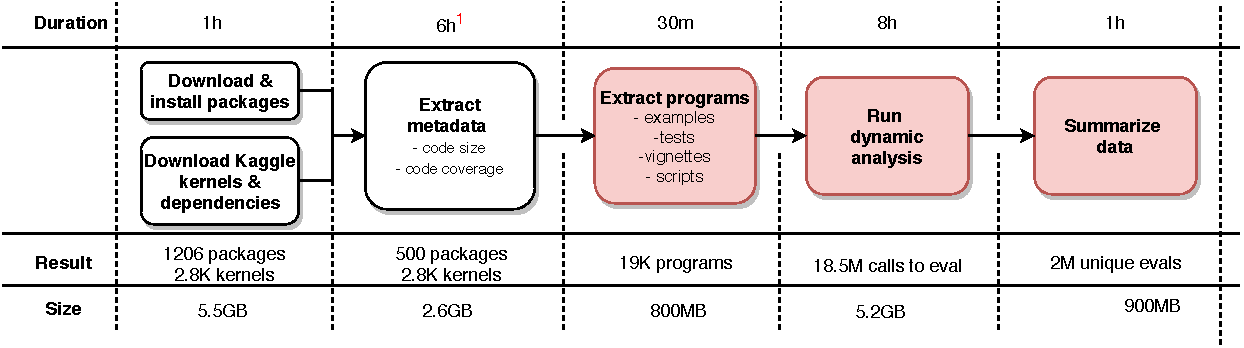
\includegraphics[width=.8\linewidth]
{pipeline.pdf}\caption{Analysis Pipeline}\label{fig:pipeline}
\end{figure*}

\medskip\emph{Discussion:~} There are two outstanding differences that set
the design of \eval in R apart from JavaScript. On the usability side, \eval
does not take a string, but an AST and an environment. This is slightly more
involved than just taking a string and may discourage some casual users.
The second substantial difference is the control that R gives over the
choice of environment in which the AST is evaluated in. Beside traditional
choices such as the top level or current lexical environment, R allows
programmers to choose a fresh, empty, environment or any environment on the
call stack. This is a significant increase in expressive power as functions
that are otherwise not aware of the use of \eval may be deeply impacted.

\section{Methodology}

\subsection{Infrastructure}

Our infrastructure consists of a dynamic analysis pipeline to record the
calls to \eval and RMarkdown notebooks for data analysis and visualization.
Figure~\ref{fig:pipeline} shows the main steps of the pipeline. We provide
the runtime, input and output data size for each step. All runs are done on
a single server Intel Xeon 6140, 2.30GHz with 72 cores and 256GB of RAM.

The pipeline begins with downloading and installing open source R packages
from CRAN for the corpus along with their dependencies. The Kaggle programs
are downloaded from \href{http://www.kaggle.com}{Kaggle} separately by a
crawler.  Next, code size and coverage metrics from the installed packages
are extracted using the \href{ https://github.com/r-lib/covr}{\covr}
package. This is followed by extraction of runnable programs from R
packages: tests, examples and vignettes as well as from Kaggle. The code of
each extracted program is wrapped into a call to dynamic analyzer
\emph{evil} (\emph{Ev}al \emph{I}nspection \emph{L}ibrary) that collects eval
usage. The reason for this is that we only want to record eval usage for the
extracted code. Without this, the data would include eval calls from the
unit testing frameworks as well as from bootstrapping R virtual machine
itself. To avoid any interference, each program is run in its own R
instance. The \emph{evil} framework is implemented as a R package in 2K lines of
R and 400 lines of C++ code.

The dynamic analyzer builds upon the dynamic analysis framework, \instrumentr
that we have implemented to enable us to write dynamic analysis logic in R. It
is an R package implemented in 2.5K lines of R and 6K lines of C++ code. It
internally uses a modified R interpreter, \rdyntrace~\cite{oopsla19a}, that
exposes hooks from within the interpreter implementation for events of interest.
\instrumentr serves as an intermediary between \rdyntrace and \evil, it
intercepts the hooks exposed by \rdyntrace and attaches R functions exported by
\evil as callbacks. The \evil callbacks execute on corresponding interpreter
events.

All steps of this pipeline are parallelized using GNU
parallel~\cite{GNUparallel} and orchestrated by GNU make. To schedule and
parallelize extraction and analysis of programs, we use the \runr
package. Furthermore, \runr gracefully handles and reports failures across
large-scale program runs which greatly aids debugging of the analysis
pipeline.  The data extracted by \evil from each program is concatenated,
cleaned and summarized in the post-processing phase by custom R
scripts. Finally, the summarized data is analyzed in RMarkdown notebooks to
gather insights. Apart from the figures, the data points included in the
paper are also generated by RMarkdown notebooks as latex macros.

\subsection{Corpus}

In this study, we report on a corpus of \CorpusCorePackages R core and
\CorpusPackages CRAN packages with \CorpusAllCodeRnd lines of source code
(native + R).  We run \CorpusAllProgramsRnd programs extracted from those
packages as well as from the user-written data-analyses shared on the Kaggle
platform. In this section we describe this corpus and methodology used to
assemble it.

\begin{figure}[!h]\centering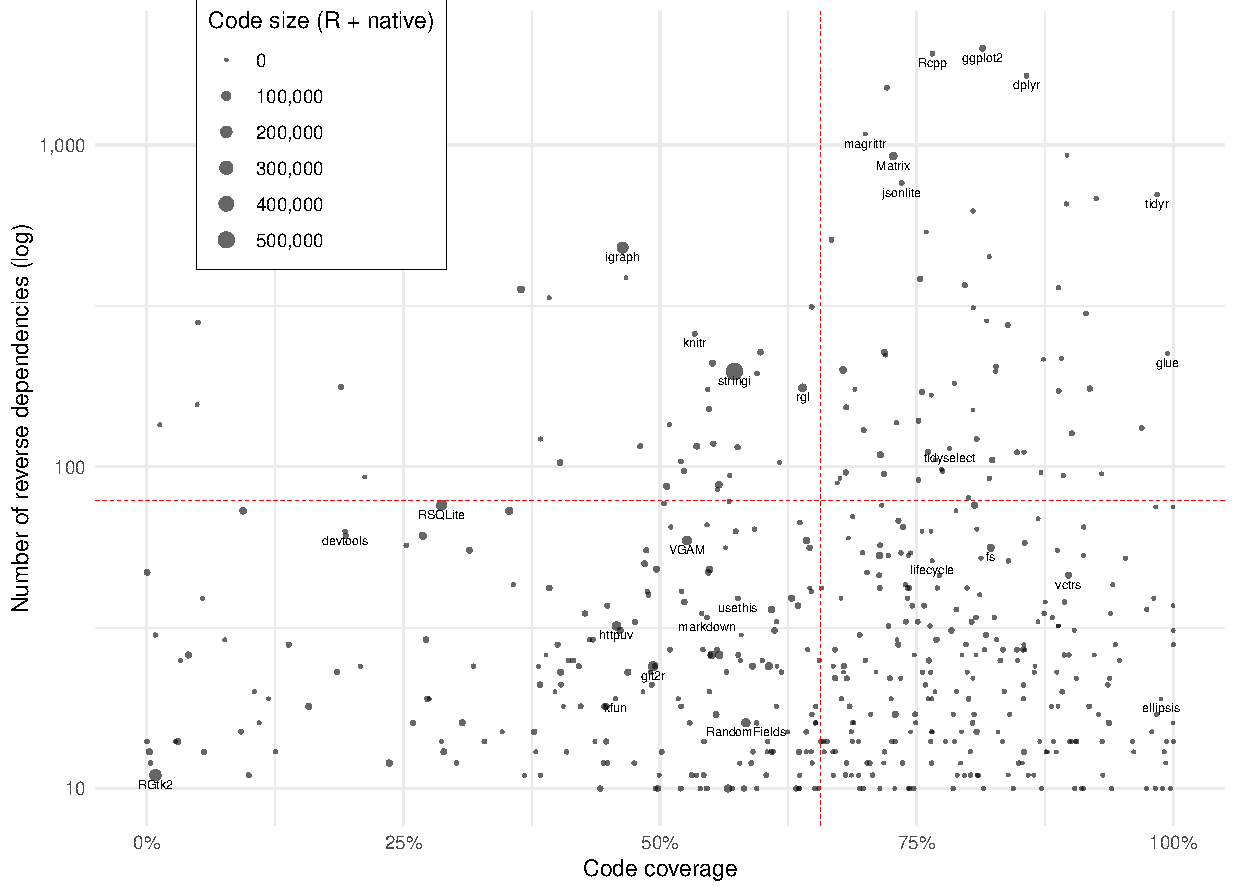
\includegraphics[width=\linewidth]
  {corpus.pdf}\caption{CRAN packages}\label{fig:corpus}
\end{figure}

\subsubsection{CRAN Packages}

We have selected the TOP \CorpusPackages packages based on their reverse
dependencies, \ie how many other packages depend on them.\footnote{Extracted
  from package metadata using a builtin function.}  This helps us find
packages which should be better written and have better code coverage.  The
resulting set contains \CorpusRCodeRnd lines of R code and
\CorpusNativeCodeRnd lines of native code.\footnote{Excluding comments and
  blank lines using \url{github.com/AlDanial/cloc}.}  For each package we
use its runnable code to compute the package code coverage.\footnote{Computed
  using \url{ https://github.com/r-lib/covr}.} On average, across the
\CorpusPackages packages, it is \CorpusMeanExprCoverage.
Figure~\ref{fig:corpus} shows these packages, the size of the dots reflects
the project's size in lines of code.  The x-axis indicates code coverage in
percents and the y-axis gives the number of call sites to \eval that were traced, in log
scale. Dotted lines indicate means. Packages with over
\CorpusEvalsPackageTreshold eval call sites are named.

All included packages come from the Comprehensive R Archive Network
(CRAN\footnote{\url{http://cran.r-project.org}}), the largest repository of R
code with over \CorpusAllCranRnd packages.\footnote{CRAN receives about 6 new
  package submissions a day~\cite{Ligges2017}.} Unlike other open code
repositories such as GitHub, CRAN is a curated repository. Each submitted
package must abide to a number of well-formedness rules that are automatically
checked asserting certain quality. Most relevant for this work is that all of
the \emph{runnable code} is tested and only a successfully running package is
admitted in the archive. This is important as we use this runnable code for the
dynamic analysis of eval calls.

There are three sources of runnable code in a R package. Next to the package
\emph{tests},\footnote{We had to exclude most tests because the {testthat}
  harness uses \eval and thus causes the entire test to register as an \eval
  call.} there are also \emph{examples} and \emph{vignettes}. Examples are R
code snippets extracted from package documentation into scripts files.
Vignettes are long-form description of package functionality written using
literate-programming style in \LaTeX\xspace or Rmarkdown with chunks of R
code that can be similarly extracted into R scripts. R provides builtin
functions for tangling the embedded code into files.  The selected packages
contain \CorpusPackagePrograms programs with \CorpusPackageProgramsCodeRnd
lines of R code: \CorpusExamplesProgramsRnd examples with
\CorpusExamplesCodeRnd lines of code, and \CorpusVignettesProgramsRnd
vignettes.

\subsubsection{Kaggle Scripts}

To represent end-user code in the corpus, we turned to Kaggle, an online
platform for data-science and machine-learning. The website allows people to
share data-science competitions, a data-analysis problem together with data,
for which users try to find the best solution. The solutions, called
{kernels}, are then shared back to the platform in the form of either plain
scripts or as notebooks.  One of the most popular competition is about
predicting passenger survival on
Titanic\footnote{\url{https://www.kaggle.com/c/titanic}} with \CorpusKaggle
kernels in R (over 1/4 of all available R kernels) which we used for our
corpus.

Unlike CRAN, Kaggle is not a curated repository and therefore there are no
guarantees about the quality of the code. After downloading all of the
\CorpusKaggle kernels and extracting the R code from the various
formats,\footnote{We use {\sf rmarkdown} to convert from notebooks to R.} we
found that \CorpusDuplicatedKaggle were whole-file duplicates. From
\CorpusRunnableKaggle kernels, \CorpusFailedKaggle failed to execute. Next
to various runtime exceptions, common problems were parse errors and
misspelled package names.  The final set contains \CorpusFinishedKaggle
kernels with \CorpusFinishedKaggleCodeRnd lines of R code.

\subsection{Threats to Validity}
The primary threat to validity is the issue of
code coverage, a cause of concern for any dynamic approach. We mitigate this
by including focusing on R packages that have high code coverage. We turn
off the bytecode compiler for this study. The bytecode compiler can also
call \eval. We do not get source locations for \UndefinedEvalsRnd eval
calls. In these cases \eval is either passed as an argument to a
higher-order functions or is defined in a function returned by a
higher-order function and the R parser does not retain location information
for \eval. However, this is a meager \PercentUndefinedEval of all eval calls
and is unlikely to affect our analysis. We ignore calls to the native \eval
function exposed by R. We also ignore the \c{rlang::tidy_eval} function
which uses native \eval internally because \c{rlang} is used to implement a
DSL for data analysis in R. It introduces a new first-class promise object
called \c{quosure} for which it implements special evaluation support in
\c{tidy_eval}.

\section{Evaluation}

This section presents the results of our empirical study of \eval in R in terms
of four research questions.

\subsection{Use of Eval}

The first research question we address is how and why \eval is used in R code.

\begin{center}{\bfseries RQ1: What are the patterns of usage of \eval in the corpus?}\end{center}

This section presents an overview of the usage of \eval in our corpus. Richards
et al. reported 82\% of JavaScript-enabled web pages using \eval~\cite{ecoop11}.
The case for R is more striking with 100\% of the programs call the \eval
function.\footnote{We combine calls to {\sf eval}, {\sf eval.parent}, {\sf
    evalq} and {\sf local}.} This high number is explained by the fact that the
R implementation, its core packages, use \eval extensively. We differentiate
three types of eval based on their origin:
%
\begin{compactitem}[$-$]
  \item a {\bf core eval} is one that occurs in the code of a core package,
  \item a {\bf dependent eval} occurs in a package imported by the target
  package, and
  \item an {\bf own eval} is one that occurs in the source code of the target
  package.
\end{compactitem}

Over all, we observe \AllAllCallCountRnd calls to \eval in our corpus.
Table~\ref{A} details this run-time information. The format is T (m/M/x)
where T is the total number of calls observed for all runs of the corpus, m
and x are the minimum and maximum number of calls for any given run, and M
is the mean number of calls per run. An average CRAN package run triggers
581 {\eval} calls in core package, 532 in dependent packages and 292 in the
CRAN package itself.  The Kaggle data set has small programs which only
trigger \eval in core and dependent packages. Thus, an average Kaggle run
has 412 core calls, 96 dependent calls, and no own calls.


%% SORRY  I HAD TO REFORMAT
\begin{table}[!h] \centering
 \begin{tabular}{r|c|c|c} \hline
Source & Core    & Dependent                      & Own \\\hline
CRAN   & 5.6M &  867K    & 259K \\
       & (1 / 337 / 46K)& (0 / 52 / 58K ) & (0 / 15 / 15K) \\\hline
Kaggle &  1.2M &  470K   & 0\\
 &  (0 / 721 / 18K) & (0 / 290 / 20K) & (0 / 0 / 0)\\\hline
\end{tabular}\caption{Eval calls in CRAN and Kaggle}\label{A}\end{table}


Table~\ref{table:site-package-summary} shows the number of call sites in
CRAN packages. \OneCallSitesEnrich{} packages have a single call site, and one
package, \emph{metafor}, has \MaxCallSitesEnrich{} call sites of
\eval. \NoCallSitesEnrich{} packages have no calls to \eval. The core packages
have \NbCoreEvalCallSites{} call sites of \eval and Kaggle has none. These
numbers are under-approximations as \eval may be called reflectively,
through aliases, or passed to a higher-order function.


\begin{table}[ht]\resizebox{\columnwidth}{!}{%
\begin{tabular}{rr|rr|rr}\hline
 Callsites & Packages & Callsites & Packages & Callsites & Packages \\\hline
% latex table generated in R 4.0.2 by xtable 1.8-4 package
% Fri Aug 28 23:16:49 2020
 1 &  61 & 6 &  12 & 11--50 &  32 \\ 
  2 &  36 & 7 &   3 & 51--100 &   6 \\ 
  3 &  15 & 8 &   4 & 101--150 &   1 \\ 
  4 &  10 & 9 &   7 &  &  \\ 
  5 &  13 & 10 &   3 &  &  \\ 
   \hline

\end{tabular}}
\caption{Distribution of callsites in CRAN}
\label{table:site-package-summary}
\end{table}

We compare the number of events intercepted during execution of \eval across
the whole corpus. For this, we use the number of interpreter steps as a
proxy for events. We observe \AllEventCountRnd events all told, and
\EvalEventCountRnd events occur inside eval (\EvalEventAllPerc of all
events). Table~\ref{table:event-distribution} shows the distribution of
events caused by \eval calls.

\begin{table}[ht]\resizebox{\columnwidth}{!}{%
\begin{tabular}{lll}\hline
Events & Core Eval Call \% & Package Eval Call \% \\ \hline
\EventsMinRangeA--\EventsMaxRangeA & \EventsCoreEvalPercA & \EventsPackageEvalPercA \\
\EventsMinRangeB--\EventsMaxRangeB & \EventsCoreEvalPercB & \EventsPackageEvalPercB \\
\EventsMinRangeC+ & \EventsCoreEvalPercC & \EventsPackageEvalPercC \\ \hline
\end{tabular}} \label{table:event-distribution}
  \caption{Events in \eval calls}
\end{table}

We observe a very wide spread in the number of events generated by \eval
calls. The largest number of events generated by an \eval call is
\EventsMaxCountRnd.  However, a majority of \eval calls performs up to
\EventsMaxRangeA events suggesting that most expressions passed to \eval are
small.  It is interesting to note that a higher proportion of Core R \eval
calls perform side effects in the \EventsMinRangeB--\EventsMaxRangeB range.
Only \EventsCoreEvalCountC Core R \eval calls and \EventsPackageEvalCountC
package \eval call generate \EventsMinRangeC to \EventsMaxRangeC events.
These \eval calls originate from statistical modeling packages such as
\mlogit, \mboost, \metafor, \lavaan, \mclust and \gamlss.


\subsubsection{A taxonomy of eval}

% Following the high-level overview of the usage of eval in the previous section,
% we now look into categorization of the eval behavior. Similarly to the JavaScript paper, we look at:
% %
% \begin{inparaenum}[(A)]
%   \item \textbf{mix} of operations performed by the expressions passed to eval,
%   \item \textbf{}
% \end{inparaenum}

In this section we turn our attention to the expression passed for evaluation to
\eval. The \eval function accepts all types of R objects as inputs, but in the
majority of cases (\AllExpressionInputEvalCallPerc), it is called with
expressions. The remaining \AllValueInputEvalCallPerc are values, \ie, they
evaluate to themselves.
%
Passing a value into an eval is effectively an no-op so we look closely at the
expression types the call sites pass to eval across all the runs.
\AllValueInputEvalSitePerc of all call sites always pass values,
\AllExpressionInputEvalSitePerc pass expressions and a very large proportion,
\AllPolymorphicInputEvalSitePerc, pass both expressions and values as inputs
across all program runs. We inspected the eval callsites that accept only values
or both values and expression as inputs. The top three of these call sites
contribute to over ~80\% of all calls to evals. The first one is inside
\c{match.arg} from core. Given a vector of names as strings, this function finds
the default values for parameters with those names in the caller function. Since
the default value for a function parameter can be a complex expression or a
benign value such as \c{NULL}, the \c{match.arg} function evaluates it through a
call to \eval. This makes the \eval inside \c{match.arg} ``polymorhpic''. The
second such \eval call originates from \ggplot, a popular R package for making
plots. \ggplot has it's own object system, \ggproto, which uses \eval inside the
\ggproto function to determine the super-class from which it inherits (the
default value is \c{NULL} but in general it could be an arbitrarily expression).
The third \eval call is in core R \c{str} function used to print a summary of R
objects. It internally maps \eval function on the bindings of an environment
which results in inputs of multiples types being passed to \eval.

We further investigate the type of input passed to \eval in
Figure~\ref{fig:eval-expression-kind} by the type of input and the source of
\eval. In this figure, \emph{Expression} is the type of program text,
\emph{Environmment} is the type of scopes or environments used for binding,
\emph{Null} is the type of the unique \c{NULL} object, \emph{Vector} is the
type assigned to vectors of strings, booleans, integers, reals and bytes;
\emph{Symbol} is the type of unevaluated symbols, and \emph{Function} is the
type of functions.

\begin{figure}[!h]
  \centering
  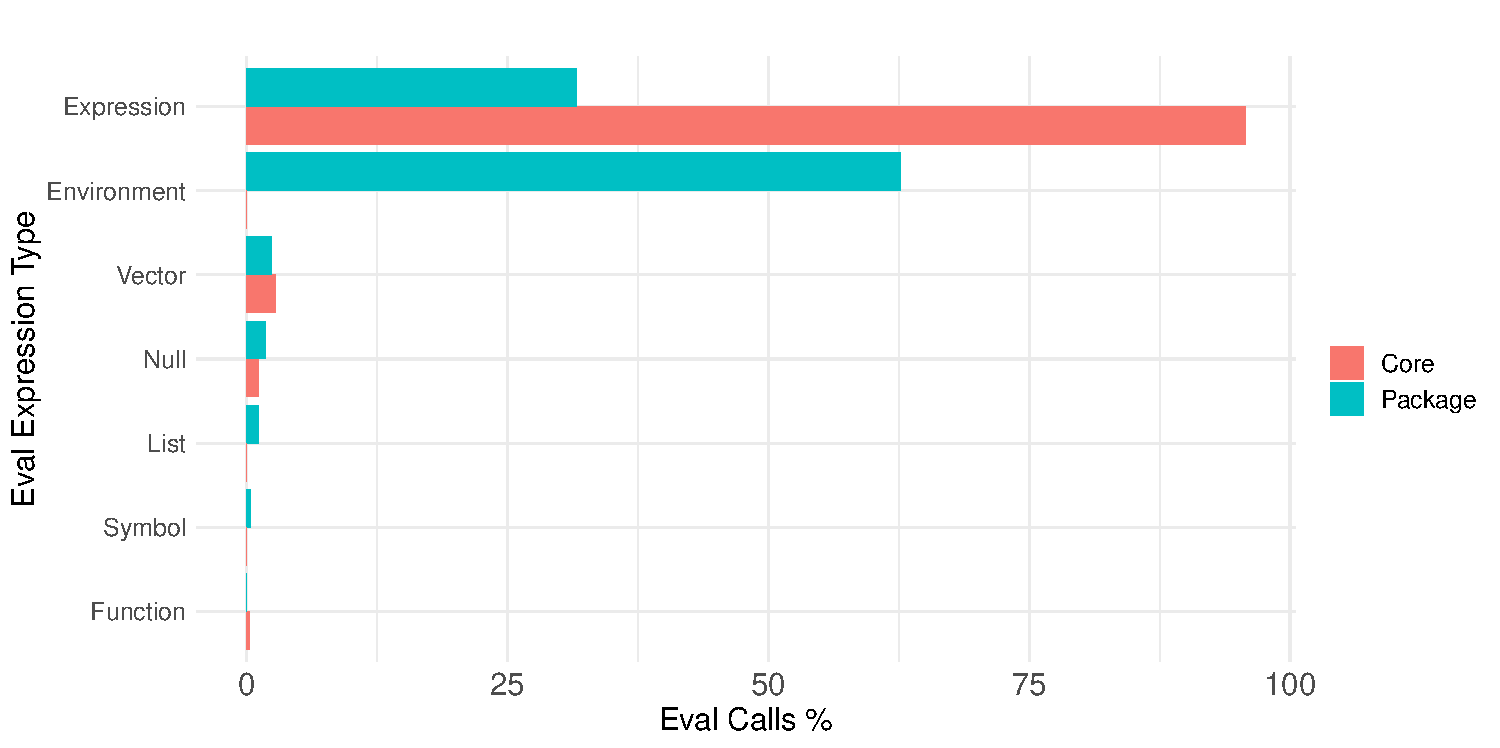
\includegraphics[width=\columnwidth]{eval-expression-kind}
  \caption{Type of Expression passed to \eval} \label{fig:eval-expression-kind}
\end{figure}

From the figure, we observe that majority of inputs to Core \eval functions
are expressions in contrast to package \eval calls which receive mostly
environments as inputs. In fact, \PackageEnvironmentInputEvalCallPerc of
\eval calls in packages receive environments as input expressions. There are
only four callsites in package evals that receive environments as
expressions.
\begin{compactitem}[$-$]
\item \c{ggplot2::ggproto} contributes to 99.9\% of package \eval calls that
  receive environments as input.
\item \c{R6::generator_funs} function contributes to only 936 \eval calls and
implements the same functionality as \c{ggplot2::ggproto} but for the \emph{R6}
OOP system.
\item \c{future::backtrace} function applies \eval to a future object which
  is implemented as an environment. This is called only once.
\item \c{RModel::str.RMmodel} function overloads the core \c{str} method for its
\c{RModel} objects and maps \eval exactly like \c{str}. This is called only
once.
\end{compactitem}

We looked at the top ten expressions passed to core and package \eval
calls. The most frequent ten expressions to eval calls from core R
contribute to 85\% of all \eval calls.

\begin{table}[!h] \centering
\begin{tabular}{@{}l|rr@{}} \hline
Expression & Eval Call &  \% \\\hline
\c{c("auto", "shell", "radix")} & 1,987,105 & 29\%\\
\c{c("auto", "shell", "quick", "radix")} & 1,593,169  & 23\%\\
\c{\{info <- loadingNamespaceInfo(...} & 1,008,632 &       14\%\\
\c{c("onLoad", "attach", "detach", "onUnload")}   & 470,566 &      6.9\%\\
\c{c("append", "prepend", "replace")} &              261,587&       3.9\% \\
\c{c("left", "right", "centre", "none")} & 162,086     & 2.4\%\\
\c{c("no", "ifany", "always")}   &                71,580 &       1.1\%\\
\c{c("pearson", "kendall", "spearman")}  & 72,962 &      1.1\%\\
\c{NULL}& 75,330  &      1.1\% \\
\c{Symbol}&                 66,279&       1\%\\\hline
\end{tabular}
\caption{Top ten eval calls in Core}\label{B}
\end{table}

The expression \c{\{info <- loadingNamespaceInfo(...} is added by core R
to a package directory during installation. To load the package, this code is
executed. It creates a namespace for the package, injects the package bindings,
and attaches the namespace to the program search path. The \c{NULL} comes from a
call to \c{substitute(subset)} in \c{stats::model.frame.default} function which
has a default value of \c{subset} as \c{NULL}. The \c{Symbol} arises from a
call to \c{as.name} in \c{base::str} function that returns a symbol that is
looked up by evaluating it in a specific environment. The remaining cases arise
from calls to \c{match.arg} which is used to look up the default choices for a
variable and match against the choice passed by the caller.

The most frequent ten expressions to eval calls from CRAN packages
contribute to 77.1\% of all \eval calls.

\begin{table}[!h]  \centering
\begin{tabular}{@{}l@{~}|@{~}r@{~}r@{}} \hline
Expression & Eval Call &  \% \\\hline
\c{Environment} &                                  989302   & 61\%\\
\c{column[rows] <<- what} &                        55677    & 3.5\%\\
\c{function(value) freduce(value, `_function_list`)} & 37251& 2.3\%\\
\c{NULL} &                         32005    & 2\%\\
\c{List} &                         22293    & 1.4\%\\
\c{c("default", "default2012", "default2011" ...}& 20610    & 1.3\%\\
\c{force(..1)}            &                        20461    & 1.3\%\\
\c{alist(`_spec`)}       &                         18532    & 1.2\%\\
\c{inner}               &                          18530    & 1.2\%\\
\c{String Vector}      &                           17487     & 1.1\%\\
\end{tabular}\caption{Top ten eval calls in CRAN} \label{C}
\end{table}

The expression \c{Environment} occurs because of the four callsites
explained above, \c{ggplot2::ggproto}, \c{R6::generator_funs},
\c{future::backtrace} and \c{RModel::str.RMmodel}. The next expression,
\c{column[rows] <<- what}, is used inside the \c{plyr::rbind.fill} function
to merge data frames by assigning concatenated vectors to rows. The \c{<<-}
operator is interesting in that it skips the current scope and assigns in a
parent scope in which the variable is already present. In our corpus, all
these \eval calls contribute to a single side-effect. The expression
\c{function(value) freduce(value, `_function_list`)} arises from the
\c{magrittr::\%>\%} function which is a pipe operator that pipes the output
of previous command to the next one. The expression is evaluated in a custom
environment to create a function binding for evaluating the components of
the pipe.\c{String Vector} and \c{List} also arise from the same function
when a string or a list is piped using the \c{\%>\%} function into the next
expression.  The \c{NULL} arises from \c{R6::generator_funs} function when
the \eval is passed a \c{NULL} argument by the \c{DataMask_generator}
package. The \c{c("default", "default2012", "default2011" ...} pattern
arises from \c{copula::polyG} where it reflectively access the default
expression for its formal parameter and evaluates it. The \c{force(..1)} and
\c{alist(`_spec`)} patterns occur in \c{glue::glue_data} function which
concatenates and interpolates strings. The two patterns occur because the
function captures unevaluated unnamed arguments and maps the evaluation of
\c{force(..1)} on them.  The \c{force} function forces promises and returns
the result of evaluation. The \c{inner} pattern arises from
\c{glue::identity_transformer} which enables the creation of custom
transformation functions for affecting the interpolation and concatenation
of input by the \c{glue} package.


\subsubsection{Operation Mix}

The JavaScript paper reported on the operation mix within \evals. This means
the proportion of read, write, and call bytecodes performed by the
JavaScript interpreter. They found that some web pages were creating objects
more frequently and writing into their fields.  In R, nearly every operation
performed in the interpreter is a function call. We observe 2.9G calls and,
of those 125M happen inside \eval (there are 463M native calls, of which
only 31M are in \eval).

{\bf there is no good reason for not counting reads and writes, we can...}


%% ...The following is fluff ...

%% Qualitatively, we observe all kinds of operations being executed inside
%% \eval calls, from numerical computing for statistical modeling to reflection
%% and metaprogramming for implementing DSLs. Even testing frameworks such
%% \c{genthat} heavily rely upon \eval to execute test code snippets. The core
%% R implementation is rife with uses of \eval for mundane things like
%% accessing default values of formal parameters and in statistical packages
%% for computation.


\subsubsection{Usage Patterns}

Richards et al.~\cite{ecoop11} identified a number of frequently occurring \eval
patterns which were detected using simple regular expressions on the \eval
strings. In the case of R we match the patterns on the recorded AST.

Table~\ref{table:js-pattens-in-r} shows the ratio of \eval in each of these
patterns. We included all the original patterns except for \emph{JSON} as R uses
its own serialization format and for \emph{empty} as there were no empty expression
passed to \eval:

\begin{table}[ht]%\resizebox{\columnwidth}{!}{%
  \centering
\begin{tabular}{r|r|r|r|r}\hline
\multirow{2}{*}{Pattern} & \multicolumn{2}{c|}{Core} & \multicolumn{2}{c}{Packages} \\
                         & Calls & Ratio            & Calls & Ratio \\\hline
% latex table generated in R 4.0.2 by xtable 1.8-4 package
% Fri Aug 28 21:43:44 2020
 Call & 6M & 93.3\% & 393.6K & 24.9\% \\ 
  Other & 402.7K & 6.3\% & 1.1M & 68.2\% \\ 
  Read & 18.4K & 0.3\% & 41.4K & 2.6\% \\ 
  Library & 3.8K & 0.06\% & 429 & 0.03\% \\ 
  Assign & 1.6K & 0.02\% & 67.2K & 4.2\% \\ 
  Try & 1.5K & 0.02\% & 41 & 0.003\% \\ 
  Typeof & 19 & 0.0003\% & 1.3K & 0.08\% \\ 
   \hline

\end{tabular}
\caption{JavaScript \eval Patterns in R}
\label{table:js-pattens-in-r}
\end{table}


\noindent \emph{Library}, \emph{Typeof} and \emph{Try} are all barely used
mostly because the language provides dedicated features for it. The few calls in
Library pattern come mostly from file loading functions such as \c{source} and
\c{sys.source}.
%
\noindent \emph{Read} pattern in JavaScript represented mostly an incorrect

access to an object's property or local variable both replaceable by
JavaScript core functions. In the case of R there are \PatternReadRnd read
\eval calls (\PatternReadRatio). They come from calls like
\c{subset(airquality, select = Temp)} where the variable \c{Temp} will be
evaluated in the \c{airquality} data frame.

%
\noindent \emph{Assign} category comprises of assignments to variables
within an \eval call. We have seen \PatternAssignRnd such calls
(\PatternAssignRatio).  \PatternAssignArrowRatio uses the simple assignment
(\c{<-}). The majority of cases comes from the \c{magrittr}'s \c{\%<>\%}
pipe operator (\PatternAssignArrowMagrittrRatio) which forwards an object to
a function on rhs and update lhs with the result. Far more calls used the
super assignment (\c{<<-}) operator, but almost all come from the \c{plyr}
package which provides a convenient API for common data manipulation
problems.
%
\noindent \emph{Call} and \emph{Other} together represents the vast majority
of eval calls in R. The \emph{Other} pattern represents all the calls where
eval was called with a value instead of with an expression. The \emph{Call}
pattern contains all the calls that did not fall in the previous
categories. Without a context it is usually difficult to further categorize
the intent of these calls.  Therefore we have randomly chosen
\PatternManualPackages packages and manually looked at
\PatternManualCallsites call sites from which we have observed the following
categories:

\subsubsection{Recording the current call} R provides a \c{match.call} function
which can return the current call. This is heavily used by the statistical
model-fitting functions that records the current call that is then
reevaluated in the different environment. Another pattern is to match the
current call, adjust some arguments and pass it to another function. For
example the \c{write.csv} function changes the \c{sep} argument in the
matched call and reevaluates itself as \c{write.table}:
%
\begin{lstlisting}
    Call <- match.call(expand.dots = TRUE)
    Call$sep <- ","; Call[[1L]] <- as.name("write.table")
    eval.parent(Call)
\end{lstlisting}

\subsubsection{Sandboxing} The combination of \eval and first class
environments can be used to construct a sandbox for evaluating
side-effecting expressions. The newly constructed environment can use the
current environment for its lexical scope. This provides the evaluated
expression access to all the bindings in the current scope but restricts the
side-effect to the newly constructed throwaway environment. However, this
sandboxing is limited because the expression can reflectively access any
environment in the call stack or use the super assignment operator(\c{<<-})
to write to parent scope. The \c{local} function which is part of Core R is
an example of this usage pattern.

\subsubsection{Dynamic Code Loading} The combination of \parse and \eval is
used to parse text from string or file and evaluate in a custom environment.
This pattern is used by the \source Core R function to load R code from a
file in the current workspace. This is quite useful for loading functions
for interactive data analysis.

\subsubsection{Metaprogramming} The combination of \eval and \substitute is
 used to do metaprogramming in R. \substitute can be used to synthesize ASTs
 by stitching together user inputs. \substitute walks over its argument AST
 and replaces the symbols with their bindings in the specified environment
 and returns this new AST which can then be evaluated in custom environments
 using \eval.

  \subsubsection{Convenience} Eval is used to make some programming tasks easier (and/or shorter). For example, in \c{data.table}, it is used to set R options from a character vector
  \begin{lstlisting}
opts = c("datatable.verbose"="FALSE", ...)
for (i in names(opts)) eval(parse(text=paste0("options(",i,"=",opts[i],")")))

  \end{lstlisting}
  %
  instead of manually calling \c{options(datatable.verbose=FALSE)}

  \subsubsection{Implementation}
  The package installation process adds an extra file to the package directory
  that contains the code to load the package code inside a \local block. It
  creates a namespace object and injects the package bindings.

  \subsubsection{Miscellaneous} \eval is also used in R packages to get around
  various limitations. For example, in \datatable package, \eval is used to
  modify a binding in the \base package of R. Bindings in the \base package are
  locked for modification and require explicit unlocking using 
  function \unlockBinding. However, directly using this function triggers a
  restricted-function-use warning during package build, preventing the package
  to be accepted by CRAN. The \datatable gets around this limitation by
  enclosing the call to \unlockBinding inside \eval. From the same reason, other
  packages use \eval to access private variables and functions from their
  dependencies.

\subsection{Necessity of Eval}

\subsubsection{Unnecessary use of eval}
  Similarly to JavaScript, there are also unnecessary uses of \eval.
  For example, the \c{PerformanceAnalytics} package contains a function
  \c{chart.QQPlot} that uses \eval to resolve a string into function and
  another to call it and assign its results into a variable:
\begin{lstlisting}
function (R, d="norm", dp, ...) {
q.f <- eval(parse(text=paste("q",d,sep="")))
z <- NULL
eval(parse(text=paste("z<-q.f(",dp,",...)")))
}
\end{lstlisting}
  In both cases, there is no need for \eval:
\begin{lstlisting}
function (R, d="norm", dp, ...) {
q.f <- get(paste0("q",d))
z <- q.f(dp, ...)
}
\end{lstlisting}
  or even to a oneliner \c{do.call(paste0("q",d), as.list(dp, ...))}.

\subsection{Power of Eval}

\subsubsection{How much code is executed inside eval}
- measure number of operations inside eval and outside eval.
- this is useful because if analyzers treat eval as a nop, they may miss X\% of the code.

\subsubsection{Does eval create observable side-effects}
- measure number of reads and writes by eval outside of its ``bubble''.
- Since R is lazy, even reads can cause promise evaluation and hence, side-effects.
- Look at writes to non-local scopes. Compare with total number of writes for
reference?
- Categorize side-effects between env passed to eval and other envs.

\subsubsection{Does eval do reflection}
\eval can access parent scopes via reflection. Find number of times it does that
and the depth to which it access parent frames.

\subsubsection{Does eval introduce new bindings}
Find number of times, eval introduces new bindings. There are many ways -- library,
load, attach, source, and explicitly introduce bindings using super-assign, assign and define.

\subsubsection{Does eval call C code}
Find number of times, eval makes call to native code using - .Call, .External,
etc. Find out if there are native functions that are called only from within eval.

\subsubsection{Does eval add finalizers}
Eval can attach code to be executed when the object goes out of scope or program
exits. Find if eval does that.

\subsubsection{Does eval do non-local returns}
Eval can do non-local returns effective bypassing evaluation of the rest of the
function. This can be useful for static analyzers.

Conclude with number of evals that are ``pure'', i.e. evals which
could be ignored by a static analyzer without any problem.

\subsubsection{Provenance}

In JavaScript, the provenance of the string passed into \eval is a matter of
concern as \eval can be used to breach the security of websites. The main
danger comes from string that were obtained from external sources. If they
are allowed to flow into an \eval, then an attacker could hijack the
program.

{\bf what have they found...}

There are various ways to obtain expressions:
\begin{itemize}
  \item \c{substitute} synthesizes ASTs from expressions by replacing
    symbols with their bindings in the specified environment.
  \item \c{expression}  creates a vector of expression
    objects from text.
  \item \c{parse}, \c{str2expression} and \c{str2lang} turn strings into
    expressions.
\end{itemize}

We observe 5.2\% cases where \eval directly evaluates the output of
\c{substitute}, 0.7\% cases where output of \c{parse} is read directly and
only 704 cases for \c{expression}. Most expressions consumed by \eval are
generated by other functions.

\c{eval(parse(...))} can be used for dynamic code loading. This forms the
core of \c{source} and \c{sys.source} functions in R that are commonly used
for loading code in R files in interactive settings. We investigated the
number of cases in which the output of \c{parse} and its variants is passed
to \eval, directly or transitively by tainting their output. This
corresponds to \PercentParsedCallSites of the total \eval call sites and
\PercentParsedEvals of the eval calls. We observed that very few of the eval
call (\NbParseFilesRnd in total) consume the result of calling \c{parse} on
a file. Most of the eval calls consume the result of calling \c{parse} on a
string.  We also identified one function in core R,
\c{invokeRestartInteractively} that prompts the user for input, parses it,
and passes it to \eval.

\subsubsection{Side-Effects}

In the corpus we observe \AllWritesRnd writes to variables of which
\EvalWritesRnd writes happen inside \eval. However, all writes are not
dangerous. Only writes to environments not local to the computation spawned
by \eval are side-effecting. These writes outlive the computation and hence
are visible outside it. The remaining writes are local to the
computation. We observe that \EvalSideEffectingWritesRnd writes inside evals
are side-effecting. This is only \EvalSideEffectingWritesEvalPerc of all
variable writes inside \eval and \EvalSideEffectingWritesAllPerc of all
variable writes in the corpus.

An \eval is considered side-effecting if it performs a side-effecting write to a
variable, directly or indirectly. Only \SideEffectingCoreCallPerc \eval calls in
Core R are side-effecting and \SideEffectingPackageCallPerc \eval calls in CRAN
packages are side-effecting.

\subsubsection{Scope}

One of the main differences of the R \eval with the javascript one is how it
interacts with \emph{scope}, or environments in R. In Javascript, \eval can
access the local scope and the global scope. In R, \eval has an argument
\c{envir} to indicate in which environment its first argument must be evaluated.
By default, it is equal to \c{parent.frame()}, 
which is the parent environment of \eval call. This default argument
happens in \DefaultEnvirExprPercent of the eval calls.

This argument can also be \c{NULL}, a \c{List} or a data frame. This happens
in 3.5\% of the cases: \eval copies the fields of the list or data frame
and creates bindings for them in a new environment. This pattern is used to
evaluate formulas which can directly refer to the fields of the data.  The
\c{envir} argument can also be a number $n$. It means that the environment
in which the expressions is evaluated will be the result of \c{sys.call(n)}
where $n$ refers to the $n$-th stack frame.

The top-level environment in R is called the global environment. New
environments can be created using \c{new.env}. They can be provided a parent
environment which becomes the enclosing scope of the new environment.

We looked at the environments passed to all the \eval calls in our corpus.
Table~\ref{tab:environments} summarizes the results. A numeric environment
class \c{n} denotes the environment of the $n$-th call stack frame from the
current function. \c{global} denotes the top-level environment and \c{list}
denotes a list passed for evaluation of formulas. Environment classes of the
form $n+$ denote the $n$-th environment extended with a new environment. The
new environment provides a limited form of sandboxing. All assignments using
the \c{\<-} function occur inside it and prevent the extended environment
from mutation. However, it is still possible to mutate the extended
environment using the \c{\<\<-} or \c{assign} functions; but, that happens
rarely.

\begin{table}[htbp] \resizebox{\columnwidth}{!}{%
    \centering
    \begin{tabular}{c|c|c|c}
        \hline
        \multicolumn{2}{c|}{Core} & \multicolumn{2}{|c}{Packages}  \\
        \hline
        Environment Class & Eval Calls \% & Environment Class & Eval Calls \% \\
        \hline
        \CoreEnvClassA & \CoreProportionA & \PackagesEnvClassA &  \PackagesProportionA\\
        \CoreEnvClassB & \CoreProportionB & \PackagesEnvClassB &  \PackagesProportionB\\
        \CoreEnvClassC & \CoreProportionC & \PackagesEnvClassC &  \PackagesProportionC\\
        \CoreEnvClassD & \CoreProportionD & \PackagesEnvClassD &  \PackagesProportionD\\
        \CoreEnvClassE & \CoreProportionE & \PackagesEnvClassE &  \PackagesProportionE\\
        \hline
    \end{tabular}} \label{tab:environments}
\caption{Environments in terms of eval calls.}
\end{table}

We observe that a disproportionately high number of core R \eval calls
access the caller's caller's environment. This is because many core R
functions call functions that pass the result of \c{parent.frame()} to an
\eval.  A disproportionately high number of calls to \eval happens in an
extended top-level environment. This can be explained by the fact that many
packages evaluate code passed from the user's workspace in the top-level
environment to access the bindings.


The \c{imchange} function of package \c{imager} makes it possible to modify
images using a dedicated formula syntax using \c{\~}.\footnote{Inspired by
 {map} in package \emph{purr}.}  Here, \eval is evaluated in \c{newenv},
which creates a new environment that inherits from \c{parent.frame()} by
default (classified as 1+).


\begin{lstlisting}
newenv <- new.env()
...
fo <- parse(text=as.character(fo)[2])
im[where] <- eval(fo,envir=newenv,enclos=env)
\end{lstlisting}

\c{adjCoef} in package \emph{actuar} find the root of an equation defined by
a function \c{h} whose arguments must be named \c{x} and \c{y}.  \c{h} is
transformed into an auxiliary function \c{h2} that can be optimized. Here,
the list used for \c{envir} ensures the correspondance between the textual
arguments of \c{h} and the arguments of \c{h2}.


\begin{lstlisting}
sh <- substitute(h)
fcall <- paste(sh, "(x, y)")
...
h2 <- function(x, y)
    eval(parse(text = fcall),
    envir = list(x = x, y = y),
    enclos = parent.frame(2))
\end{lstlisting}

\section{Discussion}

\subsection{Comparison with Javascript}

\medskip\noindent\emph{Discussion:} Comparing the use of \eval in R and
JavaScript is instructive. The use of \eval is more widespread in data
science code than it was in JavaScript. Any run of an R program seems to
trigger \eval; moreover package programmers use \eval liberally. On the
other hand, the authors of Kaggle packages do not use the feature at all.
This point to a bifurcated user community: experts who write package know
how to use \eval while end-users do not. An alternative explanation is that
end-users do not need \eval for simple data analysis tasks. This bifurcation
was not observed in the JavaScript community, but this may have changed with
the advent of Node.js ecosystem.  The distribution of input sizes is similar
to that found in JavaScript, the majority of inputs being rather small.


\begin{figure}[!b]
	\centering
  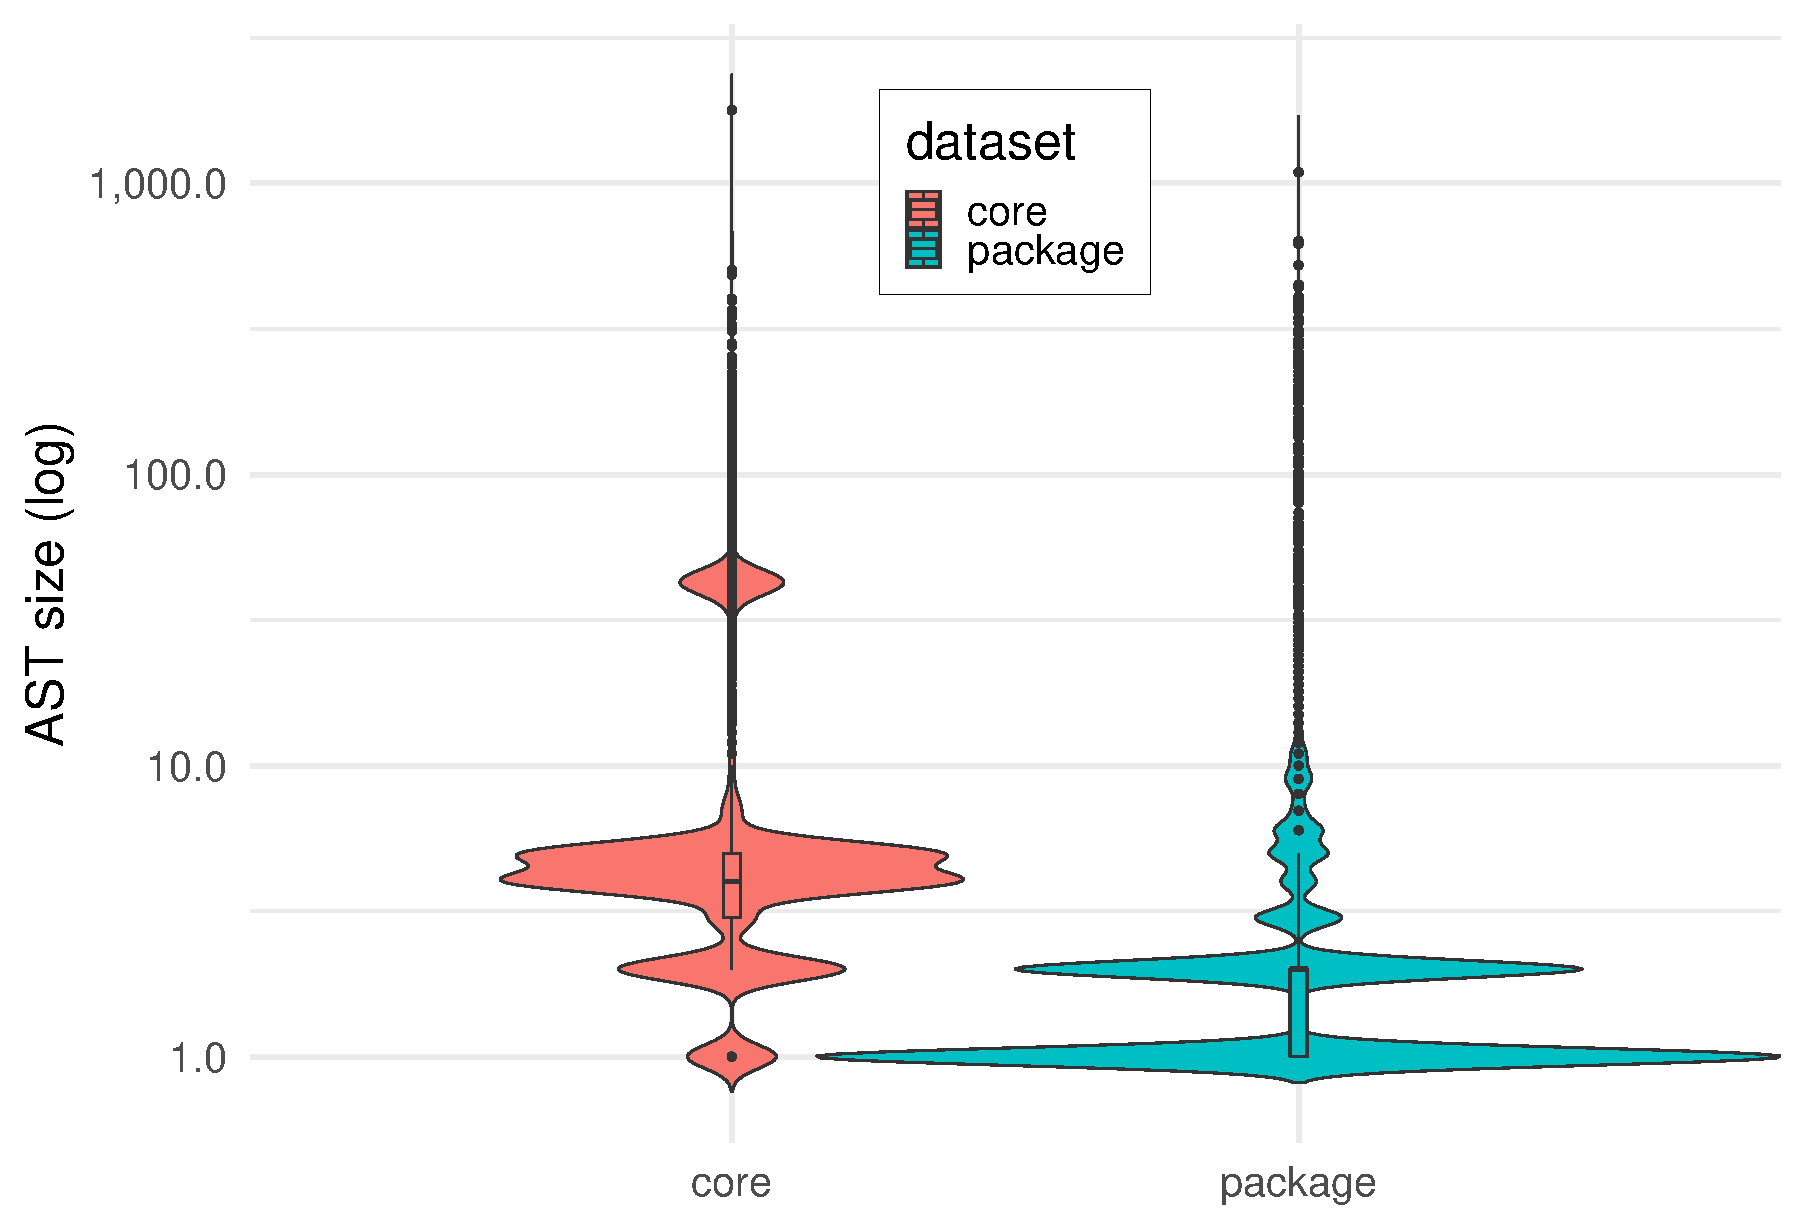
\includegraphics[width=\columnwidth]{ast_sizes}
  \caption{Input sizes} \label{fig:ast-size}
\end{figure}

To roughly estimate the complexity of the code being evaluated,
Fig.~\ref{fig:ast-size} shows the distribution of the abstract syntax tree
size of the \c{expr} argument to \eval. The majority of inputs across core
and packages (\NbAstOnePercent of \eval calls and \NbAstOneCallSitePercent
of call sites) have size 1. That is to say, the code being evaluated
consists of a single variable name or constant. A function call needs at
least three nodes and a list such as \c{c(1, 2, 3)} counts for 4
nodes. Inputs smaller than \AstSizeNineFive nodes account for 95\% of all
calls. Sizes in core are larger than in packages. Most large ASTs originate
from library \c{VGAM}, which is used for statistical modeling, and also calls functions using \eval from core. It uses
\eval to evaluate large matrices with values in a given environment.

\subsubsection{Consistency}

We look at how \emph{consistent} the \c{expr} argument of \eval can be, \ie
how many different types of the resolved \c{expr} there are per call
sites. Most of the call sites, \ie \PercentMonomorphic, are
\emph{consistent}, and this is similar to javascript. However, a few ones
are highly \emph{polymorphic} (10 different types). They are the pipe
operators \c{\%>\%}, \c{\%<>\%} and \c{\%\$\%} in package \emph{magrittr}. It
is effectively used to compose functions on their first argument, which can
be of any type.


\section{Conclusion}

\bibliography{bib/bibliography,bib/jv}

\end{document}
